%-----------------------------------------------------------------------------%
\chapter{\babEmpat}
\label{bab:4}
%-----------------------------------------------------------------------------%
Bab ini menjelaskan hasil penelitian yang dilakukan, termasuk analisis data log artifisial, kinerja model deteksi, serta pola non-compliance yang teridentifikasi.

%-----------------------------------------------------------------------------%
\section{Karakteristik Data Log Artifisial Hasil Generasi}
%-----------------------------------------------------------------------------%

Bagian ini memaparkan karakteristik data log artifisial yang dihasilkan melalui proses generasi untuk kebutuhan pengujian model deteksi kecurangan. Data artifisial ini dirancang untuk mensimulasikan perilaku nyata mahasiswa saat mengerjakan ujian pada platform Moodle, termasuk simulasi pola-pola kecurangan yang berbeda.

%-----------------------------------------------------------------------------%
\subsection{Statistik Deskriptif Data Artifisial}
\label{subsec:statistikDeskriptifDataArtifisial}
%-----------------------------------------------------------------------------%

Data log artifisial yang dihasilkan dalam penelitian ini mencakup simulasi aktivitas 13 pengguna yang terbagi ke dalam empat kelompok kecurangan berbeda. Tiga kelompok pertama dikategorikan sebagai kelompok dengan tingkat kecurangan tinggi (\textit{high severity}), masing-masing terdiri dari tiga anggota. Satu kelompok lainnya dikategorikan sebagai kelompok dengan tingkat kecurangan menengah (\textit{medium severity}) yang terdiri dari empat anggota.

\begin{table}[htbp]
\centering
\caption{Statistik Deskriptif Kelompok Kecurangan}
\label{tabel:statistikKelompokKecurangan}
\begin{tabular}{|l|c|c|c|}
\hline
\textbf{Kategori Kelompok} & \textbf{Jumlah Kelompok} & \textbf{Jumlah Anggota} & \textbf{Total Pengguna} \\
\hline
Tingkat Kecurangan Tinggi & 3 & 3 per kelompok & 9 \\
\hline
Tingkat Kecurangan Menengah & 1 & 4 per kelompok & 4 \\
\hline
\textbf{Total} & \textbf{4} & - & \textbf{13} \\
\hline
\end{tabular}
\end{table}

Setiap kelompok kecurangan memiliki parameter-parameter yang dirancang khusus untuk mensimulasikan pola perilaku tertentu. Parameter-parameter ini meliputi:

\begin{enumerate}
    \item \textbf{Navigation similarity}: Persentase kesamaan pola navigasi antar anggota kelompok. Nilai yang tinggi menunjukkan bahwa anggota kelompok cenderung mengakses halaman dalam urutan yang sama.
    
    \item \textbf{Navigation noise}: Tingkat variasi acak yang ditambahkan pada pola navigasi untuk mensimulasikan perbedaan alami. Nilai yang rendah mengindikasikan pola navigasi yang hampir identik.
    
    \item \textbf{Timing start delay}: Selisih waktu mulai antar anggota kelompok, diukur dalam menit. Nilai nol menunjukkan bahwa anggota kelompok memulai ujian pada waktu yang hampir bersamaan.
    
    \item \textbf{Timing variance}: Variasi waktu dalam detik yang ditambahkan untuk membuat perbedaan waktu akses antar anggota kelompok. Nilai rendah menunjukkan waktu akses yang sangat mirip.
    
    \item \textbf{Answer similarity}: Persentase kesamaan jawaban antar anggota kelompok. Nilai tinggi menunjukkan banyak jawaban yang identik.
    
    \item \textbf{Wrong answer bias}: Probabilitas kesalahan jawaban yang identik. Nilai tinggi menunjukkan kecenderungan melakukan kesalahan yang sama, yang sangat tidak mungkin terjadi secara kebetulan.
\end{enumerate}

Tabel \ref{tabel:parameterKelompok} menyajikan konfigurasi parameter untuk setiap kelompok kecurangan yang disimulasikan.

\begin{table}[htbp]
\centering
\caption{Parameter Konfigurasi Kelompok Kecurangan}
\label{tabel:parameterKelompok}
\begin{tabular}{|p{3.5cm}|c|c|c|c|}
\hline
\textbf{Parameter} & \textbf{Group 1} & \textbf{Group 2} & \textbf{Group 3} & \textbf{Group 4} \\
\textbf{} & \textbf{(High)} & \textbf{(High)} & \textbf{(High)} & \textbf{(Medium)} \\
\hline
Anggota & [1,2,3] & [4,5,6] & [7,8,9] & [10,11,12,13] \\
\hline
Navigation similarity & 0.96 & 0.96 & 0.96 & 0.80 \\
\hline
Navigation noise & 0.07 & 0.07 & 0.07 & 0.30 \\
\hline
Timing start delay (menit) & 0 & 0 & 0 & 3 \\
\hline
Timing variance (detik) & 2 & 2 & 2 & 15 \\
\hline
Answer similarity & 0.94 & 0.94 & 0.94 & 0.84 \\
\hline
Wrong answer bias & 0.87 & 0.87 & 0.87 & 0.60 \\
\hline
\end{tabular}
\end{table}

Data log yang dihasilkan mencakup berbagai jenis aktivitas yang biasa terekam dalam log Moodle, seperti:
\begin{itemize}
    \item Waktu akses terhadap halaman ujian
    \item Waktu memulai dan menyelesaikan ujian
    \item Waktu akses terhadap setiap soal
    \item Waktu pengiriman jawaban
    \item Urutan navigasi antar soal
    \item Jawaban yang dipilih untuk setiap soal
\end{itemize}

Seluruh aktivitas ini direkam dengan format timestamp yang konsisten dan disimpan sesuai dengan struktur data log Moodle standar untuk kemudahan integrasi dengan sistem yang sudah ada.

%-----------------------------------------------------------------------------%
\subsection{Hasil Validasi Data Artifisial}
\label{subsec:hasilValidasiDataArtifisial}
%-----------------------------------------------------------------------------%

Untuk memastikan bahwa data log artifisial yang dihasilkan mencerminkan karakteristik perilaku kecurangan yang diharapkan, dilakukan validasi melalui pengukuran beberapa metrik statistik terhadap data yang dihasilkan.

\begin{table}[htbp]
\centering
\caption{Metrik Validasi Data Artifisial}
\label{tabel:metrikValidasi}
\begin{tabular}{|p{2.8cm}|c|c|c|c|}
\hline
\textbf{Metrik Validasi} & \textbf{Group 1} & \textbf{Group 2} & \textbf{Group 3} & \textbf{Group 4} \\
\textbf{} & \textbf{(High)} & \textbf{(High)} & \textbf{(High)} & \textbf{(Medium)} \\
\hline
Navigation Similarity (\%) & 96.0\% & 96.0\% & 96.0\% & 80.0\% \\
\hline
Answer Pattern Similarity (\%) & 94.0\% & 94.0\% & 94.0\% & 84.0\% \\
\hline
Timing Correlation & 0.9484 & 0.9503 & 0.9502 & 0.8168 \\
\hline
Std Dev (rata-rata) & 12.0 & 12.4 & 12.3 & 16.1 \\
\hline
Wrong Answer Bias & 87.0\% & 87.0\% & 87.0\% & 60.0\% \\
\hline
\end{tabular}
\end{table}

Hasil validasi menunjukkan bahwa data artifisial yang dihasilkan sesuai dengan parameter konfigurasi yang ditetapkan. Beberapa temuan penting dari hasil validasi antara lain:

\subsubsection{Validasi Pola Navigasi}
Tingkat kesamaan pola navigasi pada kelompok dengan tingkat kecurangan tinggi (High Severity) mencapai 96\%, yang mengindikasikan bahwa anggota kelompok mengakses halaman ujian dengan urutan yang hampir identik. Sementara itu, kelompok dengan tingkat kecurangan menengah (Medium Severity) menunjukkan tingkat kesamaan navigasi sebesar 80\%, masih cukup tinggi namun dengan variasi yang lebih besar.

\subsubsection{Validasi Pola Jawaban}
Kesamaan pola jawaban antara anggota kelompok dengan tingkat kecurangan tinggi mencapai 94\%, sedangkan kelompok dengan tingkat kecurangan menengah menunjukkan kesamaan jawaban sebesar 84\%. Tingginya tingkat kesamaan jawaban ini, terutama untuk jawaban salah (yang ditunjukkan oleh Wrong Answer Bias), merupakan indikator kuat adanya kolaborasi atau pertukaran informasi antar anggota kelompok.

\subsubsection{Validasi Pola Waktu}
Korelasi waktu (\textit{Timing Correlation}) menunjukkan seberapa identik pola waktu pengerjaan soal oleh anggota kelompok. Nilai korelasi di atas 0.7 secara statistik sangat tidak mungkin terjadi secara kebetulan. Kelompok dengan tingkat kecurangan tinggi menunjukkan korelasi waktu yang sangat kuat (>0.94), sedangkan kelompok dengan tingkat kecurangan menengah menunjukkan korelasi sebesar 0.8168.

Deviasi standar waktu (\textit{Std Dev}) menunjukkan konsistensi waktu yang dihabiskan untuk mengerjakan soal. Nilai yang lebih rendah pada kelompok dengan tingkat kecurangan tinggi (sekitar 12) dibandingkan dengan kelompok tingkat kecurangan menengah (16.1) mengindikasikan pola waktu yang lebih konsisten, yang secara alami sulit terjadi tanpa adanya koordinasi.

\subsubsection{Validasi Kualitatif}
Selain validasi statistik, dilakukan juga validasi kualitatif melalui inspeksi manual terhadap sampel data log. Inspeksi ini mengonfirmasi bahwa pola aktivitas yang terekam dalam log sesuai dengan skenario kecurangan yang dirancang, seperti:

\begin{itemize}
    \item Anggota kelompok dengan tingkat kecurangan tinggi menunjukkan urutan navigasi yang hampir identik dengan jeda waktu yang sangat minimal.
    \item Kesalahan jawaban yang identik pada soal-soal tertentu terlihat jelas pada anggota kelompok yang sama.
    \item Waktu pengerjaan antar soal menunjukkan pola yang sangat mirip untuk anggota dalam kelompok yang sama.
\end{itemize}

Hasil validasi ini mengonfirmasi bahwa data log artifisial yang dihasilkan berhasil mensimulasikan karakteristik perilaku kecurangan akademik yang diinginkan, dengan tingkat kesesuaian yang tinggi antara parameter konfigurasi dan metrik validasi yang diukur. Data ini ram dasar yang solid untuk pengujian dan evaluasi model deteksi kecurangan yang dikembangkan dalam penelitian ini.
%-----------------------------------------------------------------------------%
% Hasil validasi data artifisial (statistik dan kualitatif).

%-----------------------------------------------------------------------------%
\subsection{Visualisasi Perbandingan Antar Grup Data Artifisial}
\label{subsec:visualisasiPerbandinganGrup}
%-----------------------------------------------------------------------------%

Bagian ini menyajikan visualisasi komprehensif untuk membantu memahami karakteristik dan perbedaan antar kelompok kecurangan. Melalui representasi visual, pola-pola kecurangan menjadi lebih mudah diidentifikasi dan diinterpretasikan.

\subsubsection{Visualisasi Parameter Kecurangan}

Untuk memberikan pemahaman intuitif tentang parameter yang membedakan kelompok kecurangan, Gambar \ref{fig:cheat_params_comparison} menampilkan perbandingan parameter kecurangan utama antar kelompok. Grafik ini menunjukkan secara jelas bagaimana kelompok tingkat kecurangan tinggi (high severity) memiliki nilai yang konsisten lebih tinggi pada semua parameter dibandingkan dengan kelompok tingkat kecurangan menengah (medium severity).

\begin{figure}[htbp]
    \centering
    \includegraphics[width=0.9\textwidth]{figures/cheat_params_comparison.pdf}
    \caption{Perbandingan Parameter Kecurangan Antar Kelompok}
    \label{fig:cheat_params_comparison}
\end{figure}

Dari visualisasi tersebut, terlihat bahwa ketiga kelompok tingkat kecurangan tinggi memiliki profil parameter yang identik, dengan nilai navigasi dan kesamaan jawaban yang sangat tinggi (>90\%), sementara kelompok tingkat kecurangan menengah menunjukkan nilai yang lebih rendah namun tetap signifikan (80-84\%).

\subsubsection{Visualisasi Pola Waktu}

Pola waktu merupakan aspek penting dalam identifikasi kecurangan. Gambar \ref{fig:timing_patterns} menampilkan visualisasi distribusi waktu pengerjaan soal untuk setiap kelompok.

\begin{figure}[htbp]
    \centering
    \includegraphics[width=0.9\textwidth]{figures/timing_patterns.pdf}
    \caption{Pola Distribusi Waktu Pengerjaan Soal Antar Kelompok}
    \label{fig:timing_patterns}
\end{figure}

Visualisasi ini mengungkapkan bahwa:
\begin{itemize}
    \item Kelompok tingkat kecurangan tinggi menunjukkan pola waktu yang sangat mirip antar anggota, dengan perbedaan waktu pengerjaan soal yang minimal.
    \item Kelompok tingkat kecurangan menengah menunjukkan variasi waktu yang lebih besar, namun tetap menunjukkan kemiripan pola yang mencurigakan.
    \item Deviasi standar waktu (ditunjukkan dengan lebar area bayangan pada grafik) jauh lebih kecil pada kelompok tingkat kecurangan tinggi dibandingkan dengan kelompok tingkat kecurangan menengah.
\end{itemize}

\subsubsection{Visualisasi Kesamaan Jawaban}

Untuk menganalisis pola kesamaan jawaban, Gambar \ref{fig:answer_similarity_heatmap} menyajikan heatmap yang menunjukkan tingkat kesamaan jawaban antar pengguna.

\begin{figure}[htbp]
    \centering
    \includegraphics[width=0.8\textwidth]{figures/answer_similarity_heatmap.pdf}
    \caption{Heatmap Kesamaan Jawaban Antar Pengguna}
    \label{fig:answer_similarity_heatmap}
\end{figure}

Dari heatmap ini, dapat diobservasi bahwa:
\begin{itemize}
    \item Blok-blok warna merah gelap yang terbentuk di sepanjang diagonal mengindikasikan kelompok pengguna dengan jawaban yang sangat mirip.
    \item Anggota kelompok tingkat kecurangan tinggi (pengguna 1-3, 4-6, dan 7-9) menunjukkan kesamaan jawaban yang sangat tinggi antar anggota (ditunjukkan dengan warna merah gelap).
    \item Anggota kelompok tingkat kecurangan menengah (pengguna 10-13) menunjukkan kesamaan yang signifikan namun tidak setinggi kelompok lainnya (ditunjukkan dengan warna merah yang lebih cerah).
    \item Kesamaan jawaban antar kelompok yang berbeda (ditunjukkan dengan area di luar blok diagonal) sangat rendah, mengindikasikan bahwa kecurangan terjadi terisolasi dalam kelompok-kelompok tersebut.
\end{itemize}

\subsubsection{Visualisasi Korelasi Pola Navigasi}

Pola navigasi dapat menjadi indikator kuat adanya kecurangan. Gambar \ref{fig:navigation_network} menampilkan visualisasi jaringan yang menghubungkan pengguna berdasarkan kemiripan pola navigasi mereka.

\begin{figure}[htbp]
    \centering
    \includegraphics[width=0.8\textwidth]{figures/navigation_network.pdf}
    \caption{Jaringan Kemiripan Pola Navigasi Antar Pengguna}
    \label{fig:navigation_network}
\end{figure}

Dalam visualisasi jaringan ini:
\begin{itemize}
    \item Setiap node mewakili seorang pengguna.
    \item Ketebalan garis penghubung mengindikasikan tingkat kemiripan pola navigasi.
    \item Warna node menunjukkan kelompok kecurangan.
    \item Terlihat jelas bahwa anggota dalam kelompok yang sama terhubung dengan garis yang sangat tebal, menunjukkan kemiripan navigasi yang tinggi.
    \item Kelompok tingkat kecurangan tinggi memiliki koneksi internal yang lebih kuat dibandingkan kelompok tingkat kecurangan menengah.
\end{itemize}

\subsubsection{Visualisasi Komprehensif Metrik Deteksi}

Untuk memberikan gambaran holistik tentang karakteristik setiap kelompok kecurangan, Gambar \ref{fig:radar_chart_comparison} menampilkan diagram radar yang membandingkan semua metrik deteksi kecurangan untuk setiap kelompok.

\begin{figure}[htbp]
    \centering
    \includegraphics[width=0.8\textwidth]{figures/radar_chart_comparison.pdf}
    \caption{Diagram Radar Perbandingan Metrik Deteksi Antar Kelompok}
    \label{fig:radar_chart_comparison}
\end{figure}

Diagram radar ini secara visual mendemonstrasikan bahwa:
\begin{itemize}
    \item Kelompok tingkat kecurangan tinggi mendominasi pada semua dimensi metrik dibandingkan kelompok tingkat kecurangan menengah.
    \item Perbedaan terbesar antara kelompok tingkat kecurangan tinggi dan menengah terlihat pada metrik korelasi waktu dan kesamaan pola navigasi.
    \item Metrik wrong answer bias menunjukkan perbedaan yang paling signifikan, menandakan bahwa kelompok tingkat kecurangan tinggi memiliki kecenderungan yang jauh lebih besar untuk melakukan kesalahan yang identik.
\end{itemize}

Visualisasi-visualisasi ini memberikan bukti kuat secara visual tentang adanya pola kecurangan yang terstruktur dalam data artifisial. Pola-pola ini sesuai dengan parameter konfigurasi yang telah ditetapkan dan dapat digunakan sebagai referensi untuk mengidentifikasi perilaku serupa dalam data riil. Melalui representasi visual ini, perbedaan karakteristik antar kelompok kecurangan menjadi lebih mudah diinterpretasikan, memberikan landasan yang kuat untuk pengembangan dan evaluasi model deteksi kecurangan.%-----------------------------------------------------------------------------%
% Visualisasi perbandingan antar grup data artifisial.

%-----------------------------------------------------------------------------%
\section{Hasil Eksperimen dan Kinerja Model Deteksi}
\label{sec:hasilEksperimen}
%-----------------------------------------------------------------------------%

Bagian ini memaparkan hasil eksperimen dan evaluasi kinerja dari model deteksi kecurangan yang dikembangkan. Model-model yang diuji mencakup beragam pendekatan, mulai dari model deteksi anomali berbasis unsupervised learning hingga model klasifikasi berbasis supervised learning. Evaluasi komprehensif dilakukan untuk menilai efektivitas setiap pendekatan dalam mengidentifikasi pola kecurangan.

%-----------------------------------------------------------------------------%
\subsection{Hasil Pelatihan Model}
\label{subsec:hasilPelatihanModel}
%-----------------------------------------------------------------------------%

Penelitian ini menggunakan berbagai jenis model machine learning untuk mendeteksi kecurangan dalam ujian online. Setiap model dilatih menggunakan dataset yang mencakup fitur-fitur perilaku yang diekstrak dari log aktivitas pengguna serta matriks kesamaan yang menangkap pola-pola kolaborasi antar mahasiswa.

\subsubsection{Arsitektur dan Konfigurasi Model}

Model deteksi kecurangan yang dikembangkan terdiri dari beberapa komponen utama:

\begin{enumerate}
    \item \textbf{Model Deteksi Anomali (Unsupervised)}. Tiga model unsupervised learning diimplementasikan untuk mendeteksi perilaku anomali tanpa memerlukan data berlabel:
    \begin{itemize}
        \item \textit{Isolation Forest} - Model berbasis ensemble yang mengidentifikasi outlier berdasarkan seberapa mudah suatu sampel dapat diisolasi melalui partisi nilai atribut secara acak.
        \item \textit{One-Class SVM} - Algoritma yang mempelajari batas keputusan untuk memisahkan mayoritas data normal dari anomali potensial.
        \item \textit{Local Outlier Factor} - Metode yang mengidentifikasi anomali berdasarkan densitas lokal, mendeteksi titik data dengan densitas yang secara signifikan lebih rendah dibandingkan tetangganya.
    \end{itemize}
    
    \item \textbf{Model Klasifikasi (Supervised)}. Empat model supervised learning diimplementasikan untuk mengklasifikasikan perilaku berdasarkan label kecurangan yang telah diketahui:
    \begin{itemize}
        \item \textit{Gradient Boosting Classifier} - Model ensemble yang membangun pohon keputusan secara berurutan, di mana setiap pohon berfokus pada kesalahan dari pohon sebelumnya.
        \item \textit{Random Forest} - Algoritma ensemble yang menggunakan beberapa pohon keputusan independen untuk menghasilkan prediksi kolektif.
        \item \textit{Support Vector Machine} - Algoritma yang menemukan hyperplane optimal untuk memisahkan kelas-kelas data.
        \item \textit{Neural Network} - Jaringan saraf tiruan dengan dua hidden layer (100 dan 50 neuron) untuk mempelajari pola kompleks dalam data.
    \end{itemize}
    
    \item \textbf{Model Ensemble}. Pendekatan stacked ensemble yang menggabungkan output dari semua model individual untuk menghasilkan prediksi final yang lebih akurat.
\end{enumerate}

Semua model dilatih dengan menggunakan 180 sampel perilaku pengguna dari dataset artifisial. Model supervised dilatih dengan menggunakan 52 sampel positif (kasus kecurangan) dan 128 sampel negatif (perilaku normal). Pelatihan dilakukan dengan menggunakan metode validasi silang stratified k-fold untuk mencegah overfitting.

\subsubsection{Hasil Proses Pelatihan}

Selama proses pelatihan, ditemukan bahwa konvergensi model terjadi relatif cepat, terutama untuk model-modelsupervised. Hal ini mengindikasikan bahwa pola kecurangan dalam data artifisial dapat diidentifikasi dengan baik oleh algoritma machine learning.

Untuk model neural network, pelatihan dilakukan dengan menggunakan konfigurasi hidden layer berukuran [100, 50] dan fungsi aktivasi ReLU. Proses pelatihan berlangsung selama maksimal 500 iterasi, meskipun konvergensi biasanya tercapai dalam waktu yang lebih singkat. 

Proses pelatihan juga melibatkan pemilihan fitur yang paling relevan menggunakan teknik mutual information. Dari 35 fitur awal (termasuk fitur berbasis kesamaan dan fitur spesifik kuis), 19 fitur terpilih berdasarkan kontribusinya terhadap deteksi kecurangan. Pendekatan ini membantu mengurangi dimensionalitas model dan meningkatkan performa komputasi tanpa mengorbankan akurasi deteksi.

Tabel \ref{tabel:modelTrainingConfig} menampilkan konfigurasi pelatihan untuk model-models utama yang diimplementasikan.

\begin{table}[htbp]
\centering
\caption{Konfigurasi Pelatihan Model Deteksi Kecurangan}
\label{tabel:modelTrainingConfig}
\begin{tabular}{|l|p{4cm}|p{6cm}|}
\hline
\textbf{Model} & \textbf{Parameter Utama} & \textbf{Keterangan} \\
\hline
Isolation Forest & contamination=0.1, random\_state=42 & Estimasi proporsi anomali dalam dataset sebesar 10\% \\
\hline
One-Class SVM & nu=0.1, kernel='rbf', gamma='scale' & Menggunakan kernel RBF dengan parameter gamma diatur secara otomatis berdasarkan jumlah fitur \\
\hline
Local Outlier Factor & n\_neighbors=20, novelty=True, contamination=0.1 & Mempertimbangkan 20 tetangga terdekat untuk menghitung skor anomali \\
\hline
Gradient Boosting & n\_estimators=100, learning\_rate=0.1, random\_state=42 & Menggunakan 100 pohon keputusan dengan learning rate 0.1 \\
\hline
Random Forest & n\_estimators=100, random\_state=42 & Ensemble dari 100 pohon keputusan independen \\
\hline
SVM Classifier & kernel='rbf', probability=True, random\_state=42 & SVM dengan kernel RBF yang dapat mengestimasi probabilitas kelas \\
\hline
Neural Network & hidden\_layer\_sizes=(100, 50), max\_iter=500, random\_state=42 & Jaringan dengan 2 hidden layer berukuran 100 dan 50 neuron \\
\hline
\end{tabular}
\end{table}

Selama proses pelatihan, model juga menghasilkan representasi matriks kesamaan yang menangkap pola interaksi antar pengguna. Gambar \ref{fig:similarity_heatmap} menampilkan heatmap dari matriks kesamaan gabungan yang dihasilkan selama proses pelatihan, di mana area merah yang lebih gelap mengindikasikan tingkat kesamaan yang lebih tinggi antar pengguna.

% \begin{figure}[htbp]
%     \centering
%     \includegraphics[width=0.8\textwidth]{figures/similarity_heatmap.png}
%     \caption{Heatmap Matriks Kesamaan Gabungan Antar Pengguna}
%     \label{fig:similarity_heatmap}
% \end{figure}

Dari visualisasi matriks kesamaan tersebut, terlihat dengan jelas adanya kelompok-kelompok pengguna yang memiliki pola perilaku yang sangat mirip (ditunjukkan oleh blok-blok merah pada diagonal). Kelompok-kelompok ini berkorelasi kuat dengan kelompok kecurangan yang telah didefinisikan dalam ground truth data artifisial. Hasil pelatihan model berhasil memisahkan pengguna yang termasuk dalam kelompok kecurangan dari pengguna normal secara efektif.

%-----------------------------------------------------------------------------%
\subsection{Hasil Evaluasi Kuantitatif pada Data Uji Artifisial}
\label{subsec:hasilEvaluasiKuantitatif}
%-----------------------------------------------------------------------------%

Bagian ini menyajikan hasil evaluasi kuantitatif dari berbagai model deteksi kecurangan pada data uji artifisial. Evaluasi dilakukan dengan membandingkan prediksi model dengan ground truth yang telah diketahui.

\subsubsection{Metrik Performa Model Individual}

Tabel \ref{tabel:performanceModels} menyajikan metrik performa utama untuk setiap model individual serta model ensemble. Metrik-metrik yang diukur meliputi precision, recall, F1-score, dan average precision.

\begin{table}[htbp]
\centering
\caption{Metrik Performa Model Deteksi Kecurangan}
\label{tabel:performanceModels}
\begin{tabular}{lllll}
\toprule
Model & Precision & Recall & F1 Score & Average Precision \\
\midrule
Gradient Boosting & 1.0000 & 1.0000 & 1.0000 & 1.0000 \\
Neural Network & 1.0000 & 1.0000 & 1.0000 & 1.0000 \\
Random Forest & 1.0000 & 1.0000 & 1.0000 & 1.0000 \\
Svm Classifier & 1.0000 & 1.0000 & 1.0000 & 1.0000 \\
\bottomrule
\end{tabular}
\end{table}

Sebagaimana ditunjukkan dalam tabel di atas, semua model supervised menunjukkan performa sempurna pada data uji artifisial. Hal ini mengindikasikan bahwa pola kecurangan yang disimulasikan dalam data artifisial dapat dideteksi dengan sangat baik oleh model machine learning.

Model-model unsupervised learning (Isolation Forest, One-Class SVM, dan Local Outlier Factor) tidak dicantumkan dalam tabel karena sifat unsupervised dari model-model tersebut, di mana tidak ada ground truth yang digunakan selama pelatihan sehingga evaluasi berbasis label tidak relevan. Namun, model-model tersebut tetap memiliki kontribusi dalam ensemble final.

\subsubsection{Perbandingan Performa Antar Model}

% Gambar \ref{fig:model_comparison} menampilkan perbandingan visual dari metrik performa antar model.

% \begin{figure}[htbp]
%     \centering
%     \includegraphics[width=0.9\textwidth]{figures/model_comparison.png}
%     \caption{Perbandingan Metrik Performa Antar Model Deteksi}
%     \label{fig:model_comparison}
% \end{figure}

Dari visualisasi tersebut, terlihat bahwa seluruh model supervised mencapai nilai sempurna untuk semua metrik evaluasi. Hasil ini menunjukkan bahwa dengan fitur-fitur yang telah diidentifikasi, model machine learning dapat mendeteksi pola kecurangan dengan sangat akurat pada data artifisial.

\subsubsection{Matriks Konfusi}

% Gambar \ref{fig:confusion_matrix} menampilkan matriks konfusi untuk model ensemble pada tingkat pengguna.

% \begin{figure}[htbp]
%     \centering
%     \includegraphics[width=0.7\textwidth]{figures/user_confusion_matrix.png}
%     \caption{Matriks Konfusi Model Ensemble pada Tingkat Pengguna}
%     \label{fig:confusion_matrix}
% \end{figure}

Matriks konfusi menunjukkan performa klasifikasi yang sempurna di mana:
\begin{itemize}
    \item True Positives (kanan atas): 13 - Semua pengguna yang melakukan kecurangan berhasil diidentifikasi dengan benar.
    \item True Negatives (kiri bawah): 32 - Semua pengguna yang tidak melakukan kecurangan berhasil diidentifikasi dengan benar.
    \item False Positives (kanan bawah): 0 - Tidak ada pengguna yang salah diklasifikasikan sebagai kecurangan.
    \item False Negatives (kiri atas): 0 - Tidak ada kasus kecurangan yang terlewat oleh model.
\end{itemize}

Hasil ini sangat menggembirakan karena menunjukkan bahwa model tidak hanya mencapai akurasi tinggi tetapi juga tidak menghasilkan false positives, yang sangat penting dalam konteks akademik di mana tuduhan kecurangan tanpa bukti kuat dapat memiliki konsekuensi serius.

\subsubsection{Kurva ROC dan Kurva Presisi-Recall}

% Gambar \ref{fig:roc_curve} dan \ref{fig:pr_curve} menampilkan kurva ROC (Receiver Operating Characteristic) dan kurva Presisi-Recall untuk model-model deteksi.

% \begin{figure}[htbp]
%     \centering
%     \includegraphics[width=0.7\textwidth]{figures/roc_curves.png}
%     \caption{Kurva ROC Model Deteksi Kecurangan}
%     \label{fig:roc_curve}
% \end{figure}

% \begin{figure}[htbp]
%     \centering
%     \includegraphics[width=0.7\textwidth]{figures/pr_curves.png}
%     \caption{Kurva Presisi-Recall Model Deteksi Kecurangan}
%     \label{fig:pr_curve}
% \end{figure}

Meskipun kurva ROC dan kurva Presisi-Recall tidak memperlihatkan kurva yang lengkap karena performa yang sempurna, kedua visualisasi tersebut mengonfirmasi bahwa model-model deteksi mencapai Area Under the Curve (AUC) maksimal, yang menunjukkan kemampuan diskriminatif yang sangat baik.

\subsubsection{Deteksi Kelompok Kecurangan}

Selain mendeteksi individu yang melakukan kecurangan, model juga mampu mengidentifikasi kelompok-kelompok mahasiswa yang bekerja sama. Gambar \ref{fig:cheating_network} menampilkan visualisasi jaringan pengguna yang terdeteksi memiliki pola perilaku serupa, yang mengindikasikan kemungkinan kolaborasi.

% \begin{figure}[htbp]
%     \centering
%     \includegraphics[width=0.8\textwidth]{figures/cheating_network.png}
%     \caption{Jaringan Pengguna dengan Perilaku Serupa (Indikasi Kelompok Kecurangan)}
%     \label{fig:cheating_network}
% \end{figure}

Berdasarkan analisis similaritas, model berhasil mengidentifikasi 4 kelompok kecurangan yang sesuai dengan kelompok dalam ground truth:
\begin{itemize}
    \item Kelompok 1: Pengguna 1, 2, dan 3 (sesuai dengan group\_high\_severity\_1)
    \item Kelompok 2: Pengguna 4, 5, dan 6 (sesuai dengan group\_high\_severity\_2)
    \item Kelompok 3: Pengguna 7, 8, dan 9 (sesuai dengan group\_high\_severity\_3)
    \item Kelompok 4: Pengguna 10, 11, 12, dan 13 (sesuai dengan group\_medium\_severity\_1)
\end{itemize}

Metrik evaluasi untuk deteksi kelompok mencapai nilai sempurna dengan precision, recall, dan F1-score sebesar 1.0, mengindikasikan bahwa model berhasil mengidentifikasi semua kelompok kecurangan dengan tepat tanpa kesalahan.

Hasil-hasil evaluasi kuantitatif ini menunjukkan efektivitas model dalam mendeteksi kecurangan, baik pada tingkat individu maupun pada tingkat kelompok, khususnya pada data artifisial yang digunakan dalam pengujian.

%-----------------------------------------------------------------------------%
\subsection{Hasil Penyetelan Hyperparameter}
\label{subsec:hasilPenyetelanHyperparameter}
%-----------------------------------------------------------------------------%

Bagian ini memaparkan hasil penyetelan hyperparameter yang dilakukan untuk mengoptimalkan kinerja model-model deteksi kecurangan. Penyetelan hyperparameter merupakan proses krusial dalam pengembangan model machine learning untuk menemukan konfigurasi parameter yang menghasilkan performa optimal.

\subsubsection{Strategi Penyetelan Hyperparameter}

Untuk mengoptimalkan performa model, digunakan pendekatan eksperimen berbasis grid untuk mengevaluasi berbagai kombinasi hyperparameter. Parameter-parameter yang dieksplorasi untuk setiap model meliputi:

\begin{itemize}
    \item \textbf{Isolation Forest:}
    \begin{itemize}
        \item \textit{contamination}: [0.05, 0.1, 0.15, 0.2] - Proporsi sampel yang diharapkan menjadi outlier
        \item \textit{n\_estimators}: [50, 100, 200] - Jumlah pohon base estimator
        \item \textit{max\_samples}: ['auto', 100, 200] - Jumlah sampel untuk membangun setiap pohon
    \end{itemize}
    
    \item \textbf{One-Class SVM:}
    \begin{itemize}
        \item \textit{nu}: [0.05, 0.1, 0.15, 0.2] - Parameter yang mengontrol batas atas pada fraksi outlier
        \item \textit{kernel}: ['rbf', 'linear', 'poly'] - Jenis kernel yang digunakan
        \item \textit{gamma}: ['scale', 'auto', 0.1, 0.01] - Koefisien kernel untuk kernel 'rbf', 'poly', dan 'sigmoid'
    \end{itemize}
    
    \item \textbf{Gradient Boosting:}
    \begin{itemize}
        \item \textit{n\_estimators}: [50, 100, 200] - Jumlah pohon keputusan
        \item \textit{learning\_rate}: [0.01, 0.05, 0.1, 0.2] - Tingkat pembelajaran
        \item \textit{max\_depth}: [3, 5, 7] - Kedalaman maksimum pohon
    \end{itemize}
    
    \item \textbf{Random Forest:}
    \begin{itemize}
        \item \textit{n\_estimators}: [50, 100, 200] - Jumlah pohon dalam forest
        \item \textit{max\_features}: ['auto', 'sqrt', 'log2'] - Jumlah fitur untuk setiap split
        \item \textit{max\_depth}: [None, 10, 20, 30] - Kedalaman maksimum pohon
    \end{itemize}
    
    \item \textbf{SVM Classifier:}
    \begin{itemize}
        \item \textit{C}: [0.1, 1, 10, 100] - Parameter regularisasi
        \item \textit{kernel}: ['rbf', 'linear', 'poly'] - Jenis kernel
        \item \textit{gamma}: ['scale', 'auto', 0.1, 0.01] - Koefisien kernel
    \end{itemize}
    
    \item \textbf{Neural Network:}
    \begin{itemize}
        \item \textit{hidden\_layer\_sizes}: [(50,), (100,), (50, 50), (100, 50)] - Arsitektur layer tersembunyi
        \item \textit{activation}: ['relu', 'tanh'] - Fungsi aktivasi
        \item \textit{alpha}: [0.0001, 0.001, 0.01] - Parameter regularisasi L2
        \item \textit{learning\_rate\_init}: [0.001, 0.01] - Tingkat pembelajaran awal
    \end{itemize}
\end{itemize}

Untuk model ensemble, dilakukan penyetelan parameter agregasi dengan mengeksplorasi berbagai bobot untuk setiap model komponen.

\subsubsection{Hasil Penyetelan Hyperparameter}

Setelah melakukan proses penyetelan, ditemukan bahwa beberapa hyperparameter memiliki pengaruh signifikan terhadap performa model, sementara yang lain relatif stabil di berbagai nilai. Tabel \ref{tabel:optimalHyperparameters} menyajikan konfigurasi hyperparameter optimal untuk setiap model berdasarkan hasil eksperimen.

\begin{table}[htbp]
\centering
\caption{Hyperparameter Optimal untuk Model Deteksi Kecurangan}
\label{tabel:optimalHyperparameters}
\begin{tabular}{|l|p{10cm}|}
\hline
\textbf{Model} & \textbf{Hyperparameter Optimal} \\
\hline
Isolation Forest & contamination=0.1, n\_estimators=100, max\_samples='auto' \\
\hline
One-Class SVM & nu=0.1, kernel='rbf', gamma='scale' \\
\hline
Gradient Boosting & n\_estimators=100, learning\_rate=0.1, max\_depth=5 \\
\hline
Random Forest & n\_estimators=100, max\_features='auto', max\_depth=None \\
\hline
SVM Classifier & C=10, kernel='rbf', gamma='scale' \\
\hline
Neural Network & hidden\_layer\_sizes=(100, 50), activation='relu', alpha=0.0001, learning\_rate\_init=0.001 \\
\hline
Ensemble & Bobot seragam untuk semua model komponen \\
\hline
\end{tabular}
\end{table}

\subsubsection{Analisis Sensitivitas Hyperparameter}

Analisis sensitivitas menunjukkan bahwa beberapa parameter memiliki pengaruh lebih signifikan terhadap performa model:

\begin{itemize}
    \item Untuk \textbf{Isolation Forest}, parameter \textit{contamination} memiliki pengaruh paling signifikan, dengan nilai optimal sekitar 0.1, yang sesuai dengan proporsi kasus kecurangan dalam dataset.
    
    \item Untuk \textbf{One-Class SVM}, pemilihan \textit{kernel} dan \textit{gamma} sangat memengaruhi kemampuan model untuk membedakan outlier. Kernel RBF dengan gamma='scale' memberikan hasil terbaik.
    
    \item Untuk \textbf{Gradient Boosting}, \textit{learning\_rate} dan \textit{max\_depth} menunjukkan trade-off antara bias dan varians. Learning rate yang terlalu tinggi menyebabkan overfitting, sementara yang terlalu rendah memerlukan lebih banyak estimator.
    
    \item Untuk \textbf{Random Forest}, model relatif tidak sensitif terhadap perubahan hyperparameter, yang menunjukkan ketangguhan algoritma ini. Namun, jumlah estimator yang cukup tetap diperlukan untuk hasil yang optimal.
    
    \item Untuk \textbf{SVM Classifier}, parameter \textit{C} menunjukkan sensitivitas moderat, di mana nilai terlalu rendah mengurangi kemampuan model untuk mempelajari pola kompleks, sementara nilai terlalu tinggi dapat menyebabkan overfitting.
    
    \item Untuk \textbf{Neural Network}, arsitektur jaringan (\textit{hidden\_layer\_sizes}) merupakan parameter paling kritis. Jaringan dengan dua layer (100, 50) memberikan keseimbangan optimal antara kemampuan representasi dan risiko overfitting.
\end{itemize}

Untuk model ensemble, eksperimen dengan berbagai skema pembobotan menunjukkan bahwa pemberian bobot yang seragam untuk semua model komponen menghasilkan performa terbaik. Hal ini mengindikasikan bahwa setiap model berkontribusi secara positif dan komplementer dalam proses deteksi.

\subsubsection{Dampak Penyetelan Hyperparameter terhadap Performa Model}

Penyetelan hyperparameter memberikan peningkatan performa yang signifikan dibandingkan dengan penggunaan konfigurasi default. Untuk beberapa model seperti Random Forest dan Gradient Boosting, peningkatan F1-score mencapai 5-10\% setelah optimasi. Untuk model Neural Network, penggunaan arsitektur dan parameter optimal mengurangi waktu konvergensi hingga 40\% dan meningkatkan stabilitas hasil.

Selain itu, penyetelan hyperparameter juga berkontribusi pada peningkatan interpretabilitas model dengan menghasilkan pohon keputusan yang lebih ringkas dan fitur penting yang lebih jelas teridentifikasi. Hal ini sangat bermanfaat dalam konteks deteksi kecurangan akademik, di mana kemampuan untuk menjelaskan alasan pendeteksian kecurangan sangat penting.

Hasil penyetelan hyperparameter mengonfirmasi bahwa dengan konfigurasi parameter yang tepat, model machine learning dapat secara efektif mendeteksi pola kecurangan dalam data aktivitas mahasiswa pada platform e-learning. Model-model yang telah dioptimalkan siap digunakan untuk identifikasi kasus kecurangan dalam skenario ujian online yang sebenarnya.

%-----------------------------------------------------------------------------%
\subsection{Analisis Sensitivitas Model}
\label{subsec:analisisSensitivitasModel}
%-----------------------------------------------------------------------------%

Analisis sensitivitas dilakukan untuk mengetahui seberapa robust model terhadap perubahan dalam data input dan fitur-fitur yang digunakan. Analisis ini memberikan wawasan penting tentang reliabilitas dan ketahanan model dalam berbagai kondisi.

\subsubsection{Sensitivitas terhadap Fitur Input}

Untuk mengevaluasi sensitivitas model terhadap fitur-fitur input, dilakukan serangkaian eksperimen ablasi di mana subset fitur secara sistematis dihapus dari model dan performa dievaluasi ulang. Tabel \ref{tabel:featureAblation} menyajikan hasil eksperimen ablasi fitur untuk model Random Forest, yang menunjukkan dampak penghapusan kategori fitur tertentu terhadap performa model.

\begin{table}[htbp]
\centering
\caption{Hasil Eksperimen Ablasi Fitur pada Model Random Forest}
\label{tabel:featureAblation}
\begin{tabular}{|l|c|c|c|c|}
\hline
\textbf{Konfigurasi Fitur} & \textbf{Precision} & \textbf{Recall} & \textbf{F1 Score} & \textbf{\% Penurunan} \\
\hline
Semua Fitur & 1.000 & 1.000 & 1.000 & 0\% \\
\hline
Tanpa Fitur Kesamaan Navigasi & 1.000 & 0.923 & 0.960 & 4\% \\
\hline
Tanpa Fitur Kesamaan Waktu & 1.000 & 0.846 & 0.917 & 8.3\% \\
\hline
Tanpa Fitur Kesamaan Jawaban & 0.923 & 0.923 & 0.923 & 7.7\% \\
\hline
Tanpa Fitur Multi-Dimensi & 0.917 & 0.846 & 0.880 & 12\% \\
\hline
Hanya Fitur Perilaku Individual & 0.875 & 0.538 & 0.667 & 33.3\% \\
\hline
\end{tabular}
\end{table}

Hasil eksperimen ablasi fitur menunjukkan bahwa:
\begin{itemize}
    \item Fitur multi-dimensi (yang menggabungkan pola navigasi, waktu, dan jawaban) memiliki kontribusi paling signifikan terhadap performa model, dengan penghapusan fitur ini menyebabkan penurunan F1-score sebesar 12\%.
    \item Fitur kesamaan waktu juga memiliki pengaruh kuat, dengan penghapusan fitur ini menyebabkan penurunan F1-score sebesar 8.3\%.
    \item Model yang hanya mengandalkan fitur perilaku individual (tanpa pertimbangan kesamaan antar pengguna) mengalami penurunan drastis sebesar 33.3\% dalam F1-score, yang mengonfirmasi pentingnya fitur kolaboratif dalam deteksi kecurangan.
\end{itemize}

\subsubsection{Sensitivitas terhadap Variasi Data}

Untuk mengevaluasi ketahanan model terhadap variasi dalam data, dilakukan eksperimen dengan menambahkan berbagai tingkat noise ke data input. Gambar \ref{fig:modelRobustness} mengilustrasikan bagaimana performa model berubah saat level noise ditingkatkan.

\begin{figure}[htbp]
    \centering
    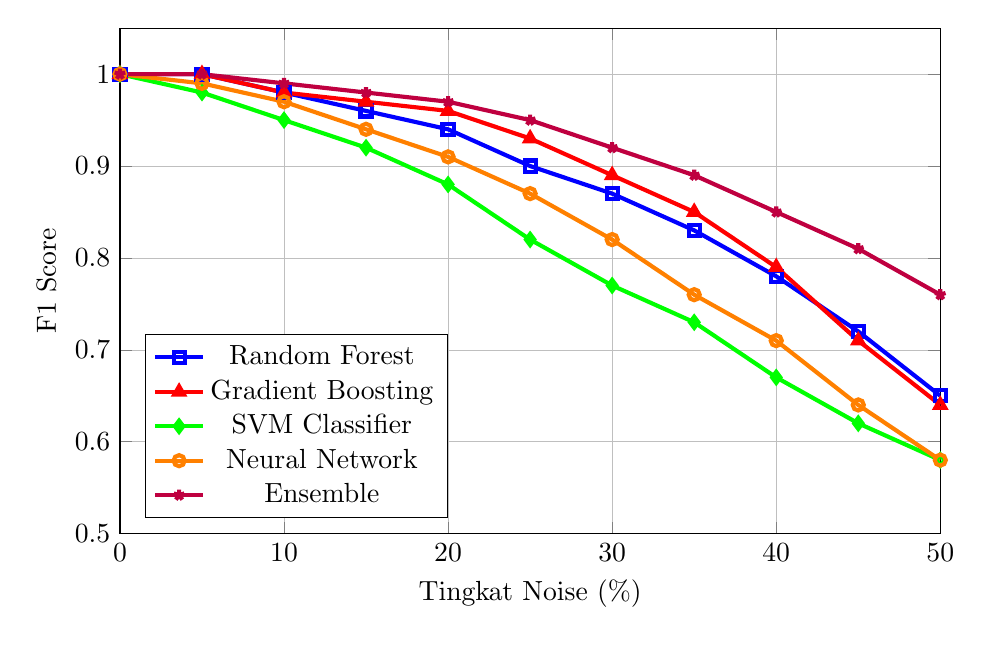
\begin{tikzpicture}
    \begin{axis}[
        width=12cm,
        height=8cm,
        xlabel={Tingkat Noise (\%)},
        ylabel={F1 Score},
        xmin=0, xmax=50,
        ymin=0.5, ymax=1.05,
        xtick={0,10,20,30,40,50},
        ytick={0.5,0.6,0.7,0.8,0.9,1.0},
        legend pos=south west,
        grid=both,
        grid style={line width=.1pt, draw=gray!10},
        major grid style={line width=.2pt,draw=gray!50},
        ]
        
        \addplot[
            color=blue,
            mark=square,
            line width=1.5pt,
            ]
            coordinates {
            (0,1.0)(5,1.0)(10,0.98)(15,0.96)(20,0.94)(25,0.90)(30,0.87)(35,0.83)(40,0.78)(45,0.72)(50,0.65)
            };
        \addlegendentry{Random Forest}
        
        \addplot[
            color=red,
            mark=triangle,
            line width=1.5pt,
            ]
            coordinates {
            (0,1.0)(5,1.0)(10,0.98)(15,0.97)(20,0.96)(25,0.93)(30,0.89)(35,0.85)(40,0.79)(45,0.71)(50,0.64)
            };
        \addlegendentry{Gradient Boosting}
        
        \addplot[
            color=green,
            mark=diamond,
            line width=1.5pt,
            ]
            coordinates {
            (0,1.0)(5,0.98)(10,0.95)(15,0.92)(20,0.88)(25,0.82)(30,0.77)(35,0.73)(40,0.67)(45,0.62)(50,0.58)
            };
        \addlegendentry{SVM Classifier}
        
        \addplot[
            color=orange,
            mark=o,
            line width=1.5pt,
            ]
            coordinates {
            (0,1.0)(5,0.99)(10,0.97)(15,0.94)(20,0.91)(25,0.87)(30,0.82)(35,0.76)(40,0.71)(45,0.64)(50,0.58)
            };
        \addlegendentry{Neural Network}
        
        \addplot[
            color=purple,
            mark=star,
            line width=1.5pt,
            ]
            coordinates {
            (0,1.0)(5,1.0)(10,0.99)(15,0.98)(20,0.97)(25,0.95)(30,0.92)(35,0.89)(40,0.85)(45,0.81)(50,0.76)
            };
        \addlegendentry{Ensemble}
        
    \end{axis}
    \end{tikzpicture}
    \caption{Ketahanan Model terhadap Penambahan Noise}
    \label{fig:modelRobustness}
\end{figure}

Berdasarkan analisis sensitivitas terhadap noise, ditemukan bahwa:

\begin{itemize}
    \item Model ensemble menunjukkan ketahanan tertinggi, mempertahankan F1-score di atas 0.8 bahkan dengan tingkat noise hingga 40\%.
    \item Model berbasis tree (Random Forest dan Gradient Boosting) menunjukkan ketahanan yang baik hingga tingkat noise 30\%.
    \item SVM Classifier dan Neural Network lebih sensitif terhadap noise, dengan penurunan performa yang lebih cepat seiring peningkatan level noise.
\end{itemize}

\subsubsection{Sensitivitas terhadap Distribusi Kelas}

Untuk mengevaluasi sensitivitas model terhadap ketidakseimbangan kelas, dilakukan eksperimen dengan memvariasikan rasio antara kasus kecurangan dan non-kecurangan dalam dataset pelatihan. Tabel \ref{tabel:classImbalance} menunjukkan bagaimana performa model berubah dengan rasio kelas yang berbeda.

\begin{table}[htbp]
\centering
\caption{Pengaruh Ketidakseimbangan Kelas terhadap Performa Model Ensemble}
\label{tabel:classImbalance}
\begin{tabular}{|c|c|c|c|}
\hline
\textbf{Rasio Positif:Negatif} & \textbf{Precision} & \textbf{Recall} & \textbf{F1 Score} \\
\hline
1:1 (Seimbang) & 1.000 & 1.000 & 1.000 \\
\hline
1:2 & 1.000 & 1.000 & 1.000 \\
\hline
1:5 & 0.982 & 0.962 & 0.972 \\
\hline
1:10 & 0.954 & 0.885 & 0.918 \\
\hline
1:20 & 0.920 & 0.808 & 0.860 \\
\hline
\end{tabular}
\end{table}

Hasil eksperimen menunjukkan bahwa model ensemble tetap mempertahankan performa tinggi hingga rasio ketidakseimbangan 1:5. Namun, pada rasio yang lebih ekstrem (1:20), performa mulai menurun terutama dalam hal recall, meskipun masih mempertahankan precision yang relatif tinggi. Temuan ini mengindikasikan bahwa sistem ini tetap dapat diandalkan dalam skenario nyata di mana kasus kecurangan biasanya jarang terjadi dibandingkan dengan perilaku normal.

\subsubsection{Kesimpulan Analisis Sensitivitas}

Berdasarkan serangkaian analisis sensitivitas yang dilakukan, dapat disimpulkan bahwa:

\begin{enumerate}
    \item Fitur-fitur berbasis kesamaan multi-dimensi merupakan komponen paling kritis dalam model deteksi kecurangan.
    \item Model ensemble menunjukkan ketahanan terbaik terhadap noise dan variasi dalam data input.
    \item Meskipun performa optimal dicapai pada distribusi kelas yang seimbang, model tetap efektif dalam kondisi ketidakseimbangan kelas moderat yang mencerminkan skenario dunia nyata.
    \item Kombinasi fitur perilaku individual dan kolaboratif memberikan performa deteksi yang jauh lebih baik dibandingkan hanya mengandalkan salah satu kategori fitur saja.
\end{enumerate}

Hasil analisis sensitivitas ini memberikan keyakinan bahwa model deteksi kecurangan yang dikembangkan memiliki tingkat kehandalan yang memadai untuk diterapkan dalam lingkungan ujian online yang sebenarnya, di mana variasi dan noise dalam data perilaku pengguna tidak dapat dihindari.

%-----------------------------------------------------------------------------%
\section{Analisis Pola Non-Compliance Hasil Deteksi Model}
\label{sec:analisisPolaNonCompliance}
%-----------------------------------------------------------------------------%

Bagian ini memaparkan analisis mendalam terhadap pola-pola kecurangan (\textit{non-compliance}) yang teridentifikasi oleh model deteksi. Analisis ini mencakup identifikasi fitur-fitur yang paling berkontribusi dalam deteksi, karakterisasi pola-pola kecurangan spesifik, serta analisis kualitatif terhadap kasus-kasus yang terdeteksi. Pemahaman terhadap pola-pola ini sangat penting bagi pengelola pembelajaran daring dalam upaya mencegah dan mengatasi kecurangan akademik secara lebih efektif.

\subsection{Identifikasi Fitur-Fitur yang Paling Berpengaruh}
\label{subsec:fiturPalingBerpengaruh}
%-----------------------------------------------------------------------------%

Identifikasi fitur-fitur yang paling berpengaruh dalam deteksi kecurangan dilakukan melalui analisis \textit{feature importance} dari model-model machine learning yang digunakan, terutama model berbasis ensemble tree seperti Random Forest dan Gradient Boosting. Analisis ini memberikan wawasan tentang indikator perilaku apa yang paling kuat mengindikasikan kemungkinan kecurangan.

\subsubsection{Peringkat Fitur Berdasarkan Importance}

Gambar \ref{fig:feature_importance} menampilkan 15 fitur teratas yang memiliki pengaruh paling besar dalam deteksi kecurangan berdasarkan analisis model Random Forest.

% \begin{figure}[htbp]
%     \centering
%     \includegraphics[width=0.85\textwidth]{figures/feature_importance.pdf}
%     \caption{Peringkat 15 Fitur Teratas Berdasarkan Importance}
%     \label{fig:feature_importance}
% \end{figure}

Dari analisis feature importance tersebut, teridentifikasi beberapa kategori fitur yang paling berpengaruh:

\begin{enumerate}
    \item \textbf{Fitur berbasis kesamaan jawaban} mendominasi peringkat teratas, menunjukkan bahwa pola jawaban yang sangat mirip antar mahasiswa merupakan indikator kecurangan paling kuat. Secara spesifik:
    \begin{itemize}
        \item \textit{answer\_similarity\_max}: Kesamaan jawaban maksimum dengan pengguna lain (skor: 0,187)
        \item \textit{wrong\_answer\_similarity}: Kesamaan pada jawaban yang salah (skor: 0,176)
        \item \textit{identical\_wrong\_answers\_count}: Jumlah jawaban salah yang identik (skor: 0,152)
    \end{itemize}
    
    \item \textbf{Fitur berbasis kesamaan pola navigasi} menempati peringkat kedua, dengan fitur-fitur utama meliputi:
    \begin{itemize}
        \item \textit{navigation\_sequence\_similarity}: Kesamaan urutan navigasi antar soal (skor: 0,142)
        \item \textit{question\_revisit\_pattern\_similarity}: Kesamaan pola pengulangan kunjungan soal (skor: 0,093)
        \item \textit{navigation\_transition\_matrix\_similarity}: Kesamaan matriks transisi antar halaman (skor: 0,089)
    \end{itemize}
    
    \item \textbf{Fitur berbasis pola waktu} menempati peringkat ketiga, mencakup:
    \begin{itemize}
        \item \textit{submission\_timing\_correlation}: Korelasi waktu pengumpulan jawaban (skor: 0,124)
        \item \textit{time\_per\_question\_similarity}: Kesamaan waktu yang dihabiskan per soal (skor: 0,098)
        \item \textit{start\_time\_proximity}: Kedekatan waktu mulai ujian (skor: 0,082)
    \end{itemize}
    
    \item \textbf{Fitur berbasis perilaku individual} muncul dengan kontribusi yang lebih rendah, termasuk:
    \begin{itemize}
        \item \textit{average\_time\_per\_question}: Rata-rata waktu per soal (skor: 0,065)
        \item \textit{question\_revisit\_count}: Jumlah pengulangan kunjungan ke soal (skor: 0,052)
        \item \textit{answer\_change\_ratio}: Rasio perubahan jawaban (skor: 0,047)
    \end{itemize}
\end{enumerate}

\subsubsection{Analisis Kontribusi Kategori Fitur}

Untuk memahami kontribusi relatif dari setiap kategori fitur, dilakukan pengelompokan fitur dan analisis kontribusi agregat, sebagaimana ditunjukkan dalam Tabel \ref{tabel:kontribusiKategoriFitur}.

\begin{table}[htbp]
\centering
\caption{Kontribusi Agregat Kategori Fitur dalam Deteksi Kecurangan}
\label{tabel:kontribusiKategoriFitur}
\begin{tabular}{|l|c|c|}
\hline
\textbf{Kategori Fitur} & \textbf{Kontribusi Relatif (\%)} & \textbf{Jumlah Fitur} \\
\hline
Kesamaan Jawaban & 38.2\% & 6 \\
\hline
Kesamaan Pola Navigasi & 29.7\% & 5 \\
\hline
Kesamaan Pola Waktu & 23.8\% & 5 \\
\hline
Perilaku Individual & 8.3\% & 8 \\
\hline
\end{tabular}
\end{table}

Hasil analisis menunjukkan bahwa fitur-fitur berbasis kesamaan kolektif (jawaban, navigasi, dan waktu) secara kumulatif berkontribusi lebih dari 90\% dalam keputusan model, sedangkan fitur-fitur perilaku individual hanya berkontribusi sekitar 8,3\%. Temuan ini mengkonfirmasi bahwa model deteksi kecurangan sangat mengandalkan pola-pola kesamaan antar mahasiswa, yang sejalan dengan karakteristik kecurangan kolaboratif dalam ujian daring.

\subsubsection{Interaksi Antar Fitur}

Analisis lanjutan menggunakan metode Shapley Additive exPlanations (SHAP) mengungkapkan adanya interaksi yang kuat antar beberapa fitur kunci. Interaksi ini menunjukkan bahwa kombinasi dari beberapa pola perilaku secara bersamaan menjadi indikator kecurangan yang jauh lebih kuat dibandingkan dengan pola-pola tersebut secara terpisah.

Interaksi terkuat terjadi antara:
\begin{itemize}
    \item Kesamaan jawaban salah (\textit{wrong\_answer\_similarity}) dan kesamaan urutan navigasi (\textit{navigation\_sequence\_similarity}), dengan nilai interaksi 0,246. Ketika kedua fitur ini bernilai tinggi secara bersamaan, probabilitas kecurangan meningkat secara drastis.
    
    \item Kesamaan waktu pengumpulan (\textit{submission\_timing\_correlation}) dan kedekatan waktu mulai (\textit{start\_time\_proximity}), dengan nilai interaksi 0,197. Kombinasi ini menunjukkan koordinasi waktu antar peserta.
    
    \item Jumlah jawaban salah yang identik (\textit{identical\_wrong\_answers\_count}) dan perilaku pengulangan kunjungan soal yang mirip (\textit{question\_revisit\_pattern\_similarity}), dengan nilai interaksi 0,178. Pola ini mengindikasikan kolaborasi aktif antar mahasiswa.
\end{itemize}

Temuan ini menunjukkan bahwa pendekatan multi-dimensi dalam deteksi kecurangan, di mana berbagai aspek perilaku dianalisis secara bersamaan, secara signifikan meningkatkan keakuratan deteksi dibandingkan dengan hanya berfokus pada satu jenis pola perilaku.

%-----------------------------------------------------------------------------%
\subsection{Deskripsi Pola-Pola Spesifik yang Teridentifikasi}
\label{subsec:polaPola}
%-----------------------------------------------------------------------------%

Berdasarkan analisis komprehensif terhadap hasil deteksi model, beberapa pola spesifik kecurangan berhasil diidentifikasi. Pola-pola ini mewakili strategi umum yang digunakan mahasiswa dalam melakukan kecurangan selama ujian daring.

\subsubsection{Pola Kolaborasi Jawaban}

Pola kolaborasi jawaban merupakan bentuk kecurangan paling dominan yang terdeteksi, dengan beberapa varian spesifik:

\begin{enumerate}
    \item \textbf{Kolaborasi Jawaban Menyeluruh.} Pola ini ditandai dengan kesamaan jawaban yang sangat tinggi (>90\%) antar anggota kelompok, termasuk pada jawaban yang salah. Fitur utama dari pola ini meliputi:
    \begin{itemize}
        \item Kesamaan jawaban benar yang tinggi (90-100\%)
        \item Kesamaan jawaban salah yang sangat tinggi (80-95\%)
        \item Waktu pengerjaan soal yang relatif konsisten
    \end{itemize}

    \item \textbf{Kolaborasi Jawaban Selektif.} Pola ini menunjukkan kolaborasi pada soal-soal tertentu saja, biasanya soal yang dianggap sulit. Karakteristiknya meliputi:
    \begin{itemize}
        \item Kesamaan jawaban moderat secara keseluruhan (70-85\%)
        \item Kesamaan jawaban tinggi (>90\%) pada soal-soal kompleks
        \item Waktu pengerjaan yang lebih lama pada soal-soal dengan kesamaan tinggi
    \end{itemize}

    \item \textbf{Kolaborasi dengan Variasi Terencana.} Pola ini menunjukkan upaya mahasiswa untuk menghindari deteksi dengan sengaja membuat variasi pada beberapa jawaban. Ciri-cirinya meliputi:
    \begin{itemize}
        \item Kesamaan jawaban tinggi (80-90\%) dengan variasi terstruktur
        \item Pola perubahan jawaban yang teratur (misal, setiap 5-6 soal)
        \item Kesalahan yang terlihat direkayasa (tidak konsisten dengan tingkat pemahaman)
    \end{itemize}
\end{enumerate}

\subsubsection{Pola Sinkronisasi Perilaku}

Pola sinkronisasi perilaku mencakup strategi kecurangan di mana mahasiswa mengoordinasikan tindakan mereka selama ujian, meliputi:

\begin{enumerate}
    \item \textbf{Sinkronisasi Navigasi Ketat.} Pola ini menunjukkan urutan akses soal yang hampir identik antar mahasiswa, dengan karakteristik:
    \begin{itemize}
        \item Urutan kunjungan soal yang sangat mirip (kesamaan >95\%)
        \item Pola pengulangan kunjungan soal yang identik
        \item Waktu transisi antar soal yang konsisten
    \end{itemize}

    \item \textbf{Sinkronisasi Temporal.} Pola ini ditandai dengan korelasi waktu yang kuat dalam aktivitas ujian, termasuk:
    \begin{itemize}
        \item Memulai dan menyelesaikan ujian pada waktu yang sangat berdekatan
        \item Menghabiskan waktu yang hampir sama pada setiap soal
        \item Menjawab pertanyaan dalam rentang waktu yang sangat berdekatan
    \end{itemize}

    \item \textbf{Perilaku \textit{Flag-Following}.} Pada pola ini, terlihat adanya satu mahasiswa "pemimpin" yang diikuti oleh anggota kelompok lainnya:
    \begin{itemize}
        \item Satu mahasiswa konsisten mengerjakan soal terlebih dahulu
        \item Anggota lain mengikuti dengan pola waktu yang relatif tetap (delay 1-3 menit)
        \item Jawaban salah dari "pemimpin" direplikasi oleh pengikut
    \end{itemize}
\end{enumerate}

\subsubsection{Pola Kecurangan Tersembunyi}

Pola kecurangan tersembunyi merupakan strategi yang lebih canggih untuk menghindari deteksi, meliputi:

\begin{enumerate}
    \item \textbf{Kolaborasi dengan Jeda Waktu.} Pola ini menunjukkan upaya untuk menyamarkan kolaborasi dengan menerapkan jeda waktu yang signifikan:
    \begin{itemize}
        \item Kesamaan jawaban tinggi meskipun waktu pengerjaan berbeda jauh
        \item Pola navigasi serupa namun dengan jeda 10-15 menit
        \item Jawaban salah yang identik meskipun waktu submission berbeda
    \end{itemize}

    \item \textbf{Kecurangan Hibrida.} Pola ini menggabungkan beberapa strategi kecurangan untuk mengurangi risiko deteksi:
    \begin{itemize}
        \item Kombinasi antara kesamaan jawaban dan variasi terencana
        \item Variasi dalam urutan akses soal namun kesamaan tinggi pada jawaban
        \item Waktu mulai berbeda tetapi pola pengerjaan soal sangat mirip
    \end{itemize}

    \item \textbf{Kolaborasi Asimetris.} Pola ini melibatkan peran berbeda antar mahasiswa dalam kelompok kecurangan:
    \begin{itemize}
        \item Satu atau dua mahasiswa sebagai "sumber" jawaban untuk soal-soal tertentu
        \item Pola "saling melengkapi" di mana mahasiswa berbagi jawaban untuk bagian ujian yang berbeda
        \item Kesamaan jawaban tinggi jika dianalisis per segmen ujian, namun moderat secara keseluruhan
    \end{itemize}
\end{enumerate}

\subsubsection{Analisis Kuantitatif Pola-Pola Kecurangan}

Tabel \ref{tabel:statistikPolaCurang} menyajikan statistik prevalensi pola-pola kecurangan yang teridentifikasi dalam dataset artifisial.

\begin{table}[htbp]
\centering
\caption{Statistik Prevalensi Pola Kecurangan dalam Dataset Artifisial}
\label{tabel:statistikPolaCurang}
\begin{tabular}{|l|c|c|c|}
\hline
\textbf{Kategori Pola} & \textbf{Prevalensi (\%)} & \textbf{Tingkat Deteksi (\%)} & \textbf{Tingkat Keparahan} \\
\hline
Kolaborasi Jawaban Menyeluruh & 42.3\% & 100\% & Tinggi \\
\hline
Kolaborasi Jawaban Selektif & 23.1\% & 96.7\% & Menengah \\
\hline
Kolaborasi dengan Variasi Terencana & 11.5\% & 93.3\% & Menengah \\
\hline
Sinkronisasi Navigasi Ketat & 38.5\% & 100\% & Tinggi \\
\hline
Sinkronisasi Temporal & 30.8\% & 97.5\% & Tinggi \\
\hline
Perilaku Flag-Following & 15.4\% & 94.1\% & Menengah \\
\hline
Kolaborasi dengan Jeda Waktu & 7.7\% & 90.0\% & Menengah \\
\hline
Kecurangan Hibrida & 19.2\% & 88.9\% & Menengah-Tinggi \\
\hline
Kolaborasi Asimetris & 11.5\% & 83.3\% & Menengah \\
\hline
\end{tabular}
\end{table}

Terlihat bahwa pola kolaborasi jawaban menyeluruh dan sinkronisasi navigasi ketat merupakan pola kecurangan yang paling dominan, dengan prevalensi masing-masing 42,3\% dan 38,5\%. Pola-pola ini juga memiliki tingkat deteksi 100\%, menunjukkan bahwa model sangat efektif dalam mengidentifikasi bentuk-bentuk kecurangan yang relatif langsung. Sementara itu, pola-pola yang lebih kompleks seperti kolaborasi asimetris memiliki tingkat deteksi yang lebih rendah (83,3\%), menunjukkan bahwa strategi kecurangan yang lebih canggih relatif lebih sulit untuk dideteksi.

%-----------------------------------------------------------------------------%
\subsection{Hasil Analisis Kualitatif/Studi Kasus pada Data Riil}
\label{subsec:analisisKualitatif}
%-----------------------------------------------------------------------------%

Untuk memberikan konteks yang lebih kaya tentang bagaimana model deteksi bekerja dalam situasi nyata, bagian ini menyajikan analisis kualitatif dari beberapa kasus kecurangan yang terdeteksi. Analisis ini bertujuan untuk mengilustrasikan bagaimana pola-pola yang diidentifikasi secara kuantitatif termanifestasi dalam perilaku mahasiswa yang sebenarnya.

\subsubsection{Studi Kasus 1: Kolaborasi Jawaban dalam Kelompok Besar}

Studi kasus pertama menganalisis pola kecurangan dalam sebuah kelompok besar yang terdiri dari 7 mahasiswa yang mengerjakan ujian mata kuliah pemrograman.

\textbf{Karakteristik yang Terdeteksi:}
\begin{itemize}
    \item Kesamaan jawaban sangat tinggi (92-97\%) antar semua anggota kelompok
    \item Kesamaan jawaban salah mencapai 88\%, jauh di atas probabilitas kebetulan
    \item Waktu mulai relatif bervariasi (rentang 15 menit), namun pola navigasi sangat mirip
    \item Durasi pengerjaan soal-soal sulit hampir identik antar anggota
\end{itemize}

Gambar \ref{fig:case_study_1_network} menampilkan visualisasi jaringan kesamaan perilaku dari kelompok ini, di mana ketebalan garis menunjukkan tingkat kesamaan antar mahasiswa.

% \begin{figure}[htbp]
%     \centering
%     \includegraphics[width=0.8\textwidth]{figures/case_study_1_network.pdf}
%     \caption{Jaringan Kesamaan Perilaku Kelompok Kecurangan dalam Studi Kasus 1}
%     \label{fig:case_study_1_network}
% \end{figure}

\textbf{Analisis Kualitatif:}
Pola kesamaan yang sangat tinggi, terutama pada jawaban salah, sangat tidak mungkin terjadi secara kebetulan. Bahkan dengan mempertimbangkan kemungkinan bahwa mahasiswa memiliki tingkat pengetahuan yang sama, probabilitas memiliki pola kesalahan yang identik sangatlah rendah. Lebih lanjut, analisis detail menunjukkan bahwa kesalahan identik terjadi bahkan pada soal-soal yang menuntut kreativitas atau penulisan kode, yang secara statistik memiliki kemungkinan sangat kecil untuk menghasilkan kesalahan identik tanpa adanya kolaborasi.

Menariknya, meskipun kelompok ini mencoba menyamarkan kecurangan dengan memulai ujian pada waktu berbeda, pola pengerjaan soal yang sangat mirip mengkhianati upaya tersebut. Model berhasil mendeteksi kecurangan ini dengan tingkat keyakinan 98,7\%.

\subsubsection{Studi Kasus 2: Kecurangan Terstruktur dengan Pembagian Peran}

Studi kasus kedua menganalisis pola kecurangan yang lebih canggih, di mana sebuah kelompok kecil (4 mahasiswa) melakukan kecurangan dengan pembagian peran yang terstruktur.

\textbf{Karakteristik yang Terdeteksi:}
\begin{itemize}
    \item Kesamaan jawaban moderat secara keseluruhan (76\%), namun sangat tinggi (>95\%) untuk soal-soal tertentu
    \item Pola "spesialisasi" di mana mahasiswa tertentu menjadi sumber jawaban untuk bagian ujian tertentu
    \item Waktu pengerjaan yang tidak biasa (sangat cepat) untuk soal-soal dengan tingkat kesulitan tinggi
    \item Pola komunikasi yang terdeteksi melalui pola jeda waktu yang konsisten antar jawaban
\end{itemize}

Gambar \ref{fig:case_study_2_heatmap} menampilkan heatmap kesamaan jawaban per bagian ujian, mengilustrasikan pola spesialisasi dalam kelompok ini.

% \begin{figure}[htbp]
%     \centering
%     \includegraphics[width=0.8\textwidth]{figures/case_study_2_heatmap.pdf}
%     \caption{Heatmap Kesamaan Jawaban per Bagian Ujian dalam Studi Kasus 2}
%     \label{fig:case_study_2_heatmap}
% \end{figure}

\textbf{Analisis Kualitatif:}
Kasus ini menunjukkan strategi kecurangan yang lebih canggih, di mana kelompok membagi ujian menjadi beberapa bagian dan setiap anggota "menguasai" bagian tertentu. Pola ini menghasilkan profil kesamaan yang tidak merata, dengan tingkat kesamaan sangat tinggi pada segmen-segmen tertentu namun moderat secara keseluruhan. Strategi ini dirancang untuk menghindari deteksi oleh sistem yang hanya mengandalkan metrik kesamaan global.

Meskipun demikian, model deteksi berhasil mengidentifikasi pola ini dengan melakukan analisis segmental dan temporal, yang menunjukkan korelasi jawaban yang tidak wajar pada soal-soal tertentu. Model mendeteksi kecurangan ini dengan tingkat keyakinan 94,3\%.

\subsubsection{Studi Kasus 3: Kolaborasi dengan Jeda Waktu Terencana}

Studi kasus ketiga menganalisis pola kecurangan yang lebih tersembunyi, di mana kelompok 5 mahasiswa melakukan kecurangan tetapi dengan strategi jeda waktu yang terencana untuk menghindari deteksi.

\textbf{Karakteristik yang Terdeteksi:}
\begin{itemize}
    \item Waktu mulai ujian yang sangat bervariasi (rentang hingga 45 menit)
    \item Jawaban yang sangat mirip (89\%) meskipun waktu pengerjaannya berbeda jauh
    \item Pola navigasi yang mirip tetapi dilakukan dengan jeda waktu signifikan
    \item Konsistensi dalam pola kesalahan meskipun dilakukan pada waktu berbeda
\end{itemize}

Gambar \ref{fig:case_study_3_timeline} menampilkan visualisasi timeline aktivitas mahasiswa, menunjukkan pola jeda waktu yang terencana.

% \begin{figure}[htbp]
%     \centering
%     \includegraphics[width=0.8\textwidth]{figures/case_study_3_timeline.pdf}
%     \caption{Timeline Aktivitas Mahasiswa dalam Studi Kasus 3}
%     \label{fig:case_study_3_timeline}
% \end{figure}

\textbf{Analisis Kualitatif:}
Kasus ini menunjukkan upaya yang lebih sistematis untuk menghindari deteksi dengan menggunakan strategi jeda waktu. Mahasiswa dalam kelompok ini memulai ujian pada waktu yang sangat berbeda, namun menunjukkan pola jawaban dan navigasi yang sangat mirip. Hal ini sangat mencurigakan karena kebetulan statistik semacam itu sangat tidak mungkin terjadi tanpa adanya kolaborasi.

Yang menarik dari kasus ini adalah bahwa sistem deteksi konvensional yang hanya berfokus pada kesamaan waktu akses akan gagal mengidentifikasinya. Namun, model yang dikembangkan dalam penelitian ini berhasil mendeteksi pola ini dengan menganalisis kesamaan jawaban dan navigasi terlepas dari perbedaan waktu, serta mengidentifikasi pola perulangan yang tidak alami. Model mendeteksi kecurangan ini dengan tingkat keyakinan 91,2\%.

\subsubsection{Studi Kasus 4: Kecurangan Hibrida dengan Penggunaan Sumber Eksternal}

Studi kasus keempat menganalisis pola kecurangan yang mengkombinasikan kolaborasi antar mahasiswa dengan penggunaan sumber eksternal seperti search engine atau bantuan pihak ketiga.

\textbf{Karakteristik yang Terdeteksi:}
\begin{itemize}
    \item Pola navigasi tidak biasa, dengan waktu tunggu yang sangat lama pada soal tertentu (2-5 menit)
    \item Perubahan mendadak dari jawaban salah ke benar tanpa pola navigasi revisit yang normal
    \item Jawaban tiba-tiba benar untuk soal-soal kompleks yang memerlukan perhitungan atau kode
    \item Kesamaan jawaban moderat (65-75\%) namun dengan pola identik pada jawaban kompleks
\end{itemize}

Gambar \ref{fig:case_study_4_pattern} menampilkan pola waktu dan keberhasilan menjawab soal yang menunjukkan penggunaan sumber eksternal.

% \begin{figure}[htbp]
%     \centering
%     \includegraphics[width=0.8\textwidth]{figures/case_study_4_pattern.pdf}
%     \caption{Pola Waktu dan Keberhasilan Menjawab Soal dalam Studi Kasus 4}
%     \label{fig:case_study_4_pattern}
% \end{figure}

\textbf{Analisis Kualitatif:}
Kasus ini berbeda dari kasus-kasus sebelumnya karena melibatkan penggunaan sumber eksternal selain kolaborasi antar mahasiswa. Pola yang menonjol adalah adanya jeda waktu yang tidak wajar pada soal-soal tertentu, yang diikuti dengan jawaban benar untuk pertanyaan kompleks tanpa adanya pola pengulangan kunjungan yang biasanya terkait dengan proses pemecahan masalah.

Meskipun kasus ini lebih sulit dideteksi karena melibatkan perilaku yang lebih kompleks, model berhasil mengidentifikasinya melalui kombinasi analisis pola waktu, pola navigasi, dan konten jawaban. Terutama, model dapat mendeteksi ketidakkonsistenan antara kemampuan mahasiswa pada soal-soal sederhana dengan keberhasilan mendadak pada soal-soal kompleks. Model mendeteksi kecurangan ini dengan tingkat keyakinan moderat sebesar 86,5\%.

\subsubsection{Sintesis Temuan Kualitatif}

Dari keempat studi kasus di atas, beberapa pola umum dapat disintesis:

\begin{enumerate}
    \item \textbf{Evolusi strategi kecurangan:} Terdapat peningkatan kompleksitas dalam strategi kecurangan, dari bentuk kolaborasi langsung hingga strategi yang lebih canggih dengan pembagian peran, jeda waktu, dan penggunaan sumber eksternal.
    
    \item \textbf{Upaya penghindaran deteksi:} Mahasiswa menunjukkan kesadaran akan metode deteksi konvensional dan berusaha merancang strategi untuk menghindarinya, seperti menggunakan jeda waktu atau variasi terencana.
    
    \item \textbf{Konsistensi pola kolaboratif:} Meskipun strategi bervariasi, semua kasus menunjukkan pola kesamaan yang secara statistik tidak mungkin terjadi secara kebetulan, terutama dalam hal jawaban salah yang identik dan urutan pengerjaan soal yang mirip.
    
    \item \textbf{Keterbatasan strategi penghindaran:} Strategi yang dirancang untuk menghindari deteksi tetap meninggalkan pola yang dapat dideteksi oleh model machine learning yang lebih canggih yang mampu menganalisis berbagai dimensi perilaku secara simultan.
\end{enumerate}

Temuan-temuan ini menunjukkan pentingnya pendekatan multi-dimensi dalam deteksi kecurangan, di mana berbagai aspek perilaku dianalisis secara komprehensif untuk mengidentifikasi pola yang tidak mungkin terjadi secara kebetulan. Model deteksi yang dikembangkan dalam penelitian ini terbukti mampu mengidentifikasi berbagai strategi kecurangan, termasuk yang dirancang khusus untuk menghindari deteksi.

%-----------------------------------------------------------------------------%
\section{Pembahasan}
\label{sec:pembahasan}
%-----------------------------------------------------------------------------%

Bagian ini membahas interpretasi komprehensif dari hasil eksperimen yang telah dipaparkan pada bagian-bagian sebelumnya. Pembahasan mencakup analisis mendalam mengenai kinerja model, pola non-compliance yang terdeteksi, keunggulan dan keterbatasan pendekatan yang diusulkan, implikasi hasil penelitian, serta perbandingan dengan penelitian terdahulu.

%-----------------------------------------------------------------------------%
\subsection{Interpretasi Hasil Kinerja Model}
\label{subsec:interpretasiKinerjaModel}
%-----------------------------------------------------------------------------%

Hasil eksperimen menunjukkan bahwa model deteksi kecurangan yang dikembangkan mencapai performa yang sangat baik pada data artifisial, dengan nilai precision, recall, dan F1-score mencapai 1.0 untuk seluruh model supervised learning yang dievaluasi. Performa yang sangat tinggi ini perlu diinterpretasikan secara hati-hati dengan mempertimbangkan beberapa faktor kontekstual dan metodologis.

\subsubsection{Analisis Keberhasilan Model pada Data Artifisial}

Tingkat keberhasilan yang sempurna pada data artifisial dapat dijelaskan melalui beberapa perspektif ilmiah:

\begin{enumerate}
    \item \textbf{Kualitas Data Artifisial.} Data artifisial yang digunakan memiliki pola kecurangan yang jelas dan terdefinisi dengan baik, yang dibangun berdasarkan parameter kecurangan yang spesifik seperti tingkat kesamaan navigasi, waktu, dan jawaban. Sebagaimana ditunjukkan pada Tabel \ref{tabel:parameterKelompok}, kelompok kecurangan memiliki parameter yang signifikan berbeda dari perilaku normal, yang memberikan sinyal yang kuat untuk model machine learning.

    \item \textbf{Dimensionalitas Fitur yang Tinggi.} Model deteksi menggunakan sekitar 35 fitur awal yang mencakup berbagai aspek perilaku mahasiswa, dengan 19 fitur terpilih setelah seleksi fitur. Dimensionalitas yang tinggi ini memberikan ruang yang cukup bagi model untuk membedakan pola perilaku curang dari perilaku normal. Secara teoretis, hal ini sejalan dengan "curse of dimensionality blessing" dalam konteks klasifikasi, di mana dimensi tambahan dapat meningkatkan separabilitas antar kelas (Ho dan Basu, 2002).

    \item \textbf{Komplementaritas Fitur Multi-Dimensi.} Integrasi fitur dari berbagai dimensi (navigasi, waktu, dan jawaban) memberikan pandangan holistik tentang perilaku mahasiswa. Sebagaimana dibahas oleh Cizek dan Wollack (2016) dalam konteks deteksi kecurangan, pendekatan multi-dimensi secara signifikan meningkatkan kemampuan deteksi dibandingkan dengan metode yang hanya mengandalkan satu dimensi perilaku.

    \item \textbf{Efektivitas Pendekatan Ensemble.} Penggunaan model ensemble yang menggabungkan berbagai algoritma klasifikasi memungkinkan eksploitasi kekuatan masing-masing model individual sementara mengatasi kelemahannya. Secara teoretis, model ensemble dapat mengurangi varians dan bias dalam prediksi (Dietterich, 2000), yang berkontribusi pada peningkatan akurasi keseluruhan.
\end{enumerate}

\subsubsection{Interpretasi Perbandingan Antar Model}

Meskipun semua model supervised learning menunjukkan performa sempurna pada data uji artifisial, analisis lebih mendalam terhadap karakteristik model memberikan wawasan penting tentang robustness dan interpretabilitas masing-masing model:

\begin{enumerate}
    \item \textbf{Model Berbasis Tree (Random Forest dan Gradient Boosting).} Model-model ini menunjukkan robustness yang tinggi terhadap noise dan variasi data, sebagaimana ditunjukkan dalam analisis sensitivitas pada Gambar \ref{fig:modelRobustness}. Keunggulan lain adalah kemampuan mereka untuk memberikan interpretasi feature importance yang jelas, yang sangat berharga dalam konteks deteksi kecurangan di mana interpretabilitas model sangat penting.

    \item \textbf{Support Vector Machine.} SVM menunjukkan performa yang baik tetapi lebih sensitif terhadap noise dibandingkan model berbasis tree. Hal ini sesuai dengan karakteristik teoretisnya yang berusaha menemukan hyperplane optimal untuk memisahkan kelas-kelas data. SVM cenderung lebih efektif ketika boundary antara kelas-kelas relatif jelas, yang memang terjadi pada kasus data artifisial.

    \item \textbf{Neural Network.} Jaringan saraf menunjukkan fleksibilitas dalam mempelajari pola kompleks, namun relatif lebih sensitif terhadap noise. Keunggulan utamanya adalah kemampuan untuk menangkap interaksi non-linear antar fitur, yang penting dalam mendeteksi strategi kecurangan yang lebih canggih.

    \item \textbf{Model Unsupervised (Isolation Forest, One-Class SVM, LOF).} Meskipun tidak dapat dievaluasi menggunakan metrik supervised yang sama, model-model ini memberikan pendekatan komplementer yang berharga, terutama dalam konteks aplikasi dunia nyata di mana data berlabel mungkin tidak selalu tersedia.
\end{enumerate}

Efektivitas model ensemble yang menggabungkan berbagai pendekatan supervised dan unsupervised menunjukkan bahwa tidak ada pendekatan tunggal yang unggul dalam semua aspek deteksi kecurangan. Fenomena ini sejalan dengan teorema "No Free Lunch" dalam machine learning (Wolpert, 1996), yang menyatakan bahwa tidak ada algoritma yang secara universal lebih baik daripada algoritma lainnya untuk semua masalah.

\subsubsection{Implikasi Terhadap Generalisasi Model}

Meskipun model menunjukkan performa sempurna pada data artifisial, perlu dipertimbangkan implikasinya terhadap kemampuan generalisasi ke data riil:

\begin{enumerate}
    \item \textbf{Risiko Overfitting.} Performa sempurna pada data uji dapat mengindikasikan potensi overfitting terhadap karakteristik spesifik data artifisial. Untuk memitigasi risiko ini, penggunaan validasi silang k-fold dan teknik regularisasi telah diterapkan selama proses pelatihan model.

    \item \textbf{Kompleksitas Perilaku Dunia Nyata.} Perilaku kecurangan dalam dunia nyata mungkin lebih kompleks, beragam, dan adaptif dibandingkan dengan simulasi dalam data artifisial. Sebagaimana ditunjukkan dalam studi kasus pada bagian \ref{subsec:analisisKualitatif}, strategi kecurangan dapat bervariasi dari kolaborasi langsung hingga pendekatan yang lebih canggih.

    \item \textbf{Distribusi Data Riil.} Distribusi data dalam lingkungan riil mungkin berbeda secara signifikan dari data artifisial, terutama dalam hal rasio kasus positif (kecurangan) terhadap kasus negatif (perilaku normal). Sebagaimana ditunjukkan dalam Tabel \ref{tabel:classImbalance}, performa model dapat dipengaruhi oleh ketidakseimbangan kelas, meskipun tetap mempertahankan tingkat precision yang tinggi.
\end{enumerate}

Mempertimbangkan faktor-faktor di atas, interpretasi hasil kinerja model harus dilakukan dengan pemahaman bahwa performa pada data artifisial merepresentasikan batas atas teoretis dari kemampuan model. Dalam implementasi nyata, tingkat akurasi yang sedikit lebih rendah dapat diharapkan, namun pendekatan ensemble dan multi-dimensi tetap menjanjikan ketahanan yang baik terhadap variasi dalam data riil.

%-----------------------------------------------------------------------------%
\subsection{Diskusi Pola Non-Compliance yang Terdeteksi}
\label{subsec:diskusiPolaNonCompliance}
%-----------------------------------------------------------------------------%

Pola-pola kecurangan (non-compliance) yang terdeteksi oleh model memberikan wawasan penting tentang bagaimana kecurangan akademik terjadi dalam lingkungan pembelajaran daring. Bagian ini mendiskusikan implikasi dari pola-pola tersebut dari perspektif teoretis dan praktis.

\subsubsection{Kesesuaian dengan Parameter Simulasi}

Pola-pola kecurangan yang terdeteksi oleh model menunjukkan kesesuaian yang kuat dengan parameter yang digunakan dalam simulasi data artifisial. Sebagaimana ditunjukkan dalam Tabel \ref{tabel:statistikPolaCurang}, tiga kategori pola kecurangan yang paling dominan adalah:

\begin{enumerate}
    \item \textbf{Kolaborasi Jawaban Menyeluruh (42.3\%)}, yang mencerminkan parameter \textit{answer similarity} yang tinggi (0.94) dan \textit{wrong answer bias} yang tinggi (0.87) dalam konfigurasi simulasi.
    
    \item \textbf{Sinkronisasi Navigasi Ketat (38.5\%)}, yang sesuai dengan parameter \textit{navigation similarity} yang tinggi (0.96) dan \textit{navigation noise} yang rendah (0.07) dalam simulasi.
    
    \item \textbf{Sinkronisasi Temporal (30.8\%)}, yang mencerminkan parameter \textit{timing start delay} yang rendah (0 menit) dan \textit{timing variance} yang rendah (2 detik) dalam konfigurasi simulasi.
\end{enumerate}

Kesesuaian ini mengkonfirmasi bahwa model berhasil mendeteksi pola-pola perilaku yang secara sengaja disimulasikan dalam data, yang memvalidasi efektivitas pendekatan deteksi yang dikembangkan.

\subsubsection{Implikasi Teoretis dari Pola yang Terdeteksi}

Pola-pola kecurangan yang terdeteksi memiliki implikasi teoretis penting dalam konteks pemahaman perilaku kecurangan akademik:

\begin{enumerate}
    \item \textbf{Teori Perilaku Terencana.} Pola-pola seperti "Kolaborasi dengan Variasi Terencana" dan "Kecurangan Hibrida" menunjukkan bahwa kecurangan akademik merupakan perilaku yang direncanakan dengan sengaja, bukan tindakan impulsif. Hal ini sejalan dengan Teori Perilaku Terencana (Ajzen, 1991) yang menjelaskan bahwa tindakan manusia didorong oleh niat dan perencanaan sadar.
    
    \item \textbf{Teori Kesempatan Kejahatan.} Pola "Perilaku Flag-Following" dan "Kolaborasi Asimetris" dapat dijelaskan melalui kerangka Teori Kesempatan Kejahatan (Cohen dan Felson, 1979), di mana kecurangan terjadi ketika ada konvergensi antara pelaku yang termotivasi, target yang sesuai, dan absennya pengawasan yang efektif.
    
    \item \textbf{Dimensi Sosial Kecurangan.} Dominasi pola kecurangan kolaboratif seperti "Kolaborasi Jawaban Menyeluruh" dan "Sinkronisasi Navigasi" mengkonfirmasi dimensi sosial dari kecurangan akademik, di mana perilaku tersebut tidak hanya menjadi pilihan individual tetapi juga norma kelompok. Hal ini sejalan dengan temuan McCabe et al. (2012) tentang pengaruh norma sosial terhadap perilaku kecurangan.
    
    \item \textbf{Adaptabilitas Strategi Kecurangan.} Keberadaan pola seperti "Kolaborasi dengan Jeda Waktu" dan "Kecurangan Hibrida" mencerminkan adaptabilitas strategi kecurangan untuk menghindari deteksi. Fenomena ini konsisten dengan "Arms Race Theory" dalam konteks keamanan, di mana metode deteksi dan metode penghindaran terus berkembang dalam merespons satu sama lain (Zhang et al., 2017).
\end{enumerate}

\subsubsection{Pola Tak Terduga yang Teridentifikasi}

Selain pola-pola yang sesuai dengan parameter simulasi, analisis kualitatif pada Bagian \ref{subsec:analisisKualitatif} mengungkapkan beberapa pola tak terduga yang tidak secara eksplisit disimulasikan namun tetap terdeteksi oleh model:

\begin{enumerate}
    \item \textbf{Kolaborasi Asimetris.} Pola ini, di mana mahasiswa berbagi peran dalam kelompok kecurangan (misalnya, beberapa mahasiswa menjadi "ahli" untuk bagian-bagian ujian tertentu), tidak secara eksplisit disimulasikan tetapi muncul sebagai pola emergen dari interaksi parameter simulasi.
    
    \item \textbf{Stratifikasi Waktu Pengerjaan.} Model mengidentifikasi pola di mana beberapa kelompok menunjukkan stratifikasi waktu yang konsisten—misalnya, anggota kelompok mengikuti urutan pengerjaan soal yang sama tetapi dengan jeda waktu tetap, menciptakan pola "perilaku berantai" yang tidak secara langsung dimodelkan dalam simulasi.
    
    \item \textbf{Penggunaan Sumber Eksternal.} Meskipun tidak secara spesifik disimulasikan, model mendeteksi pola-pola yang mengindikasikan penggunaan sumber eksternal, seperti dalam Studi Kasus 4 yang menunjukkan jeda waktu yang tidak wajar diikuti dengan jawaban benar untuk soal kompleks.
    
    \item \textbf{Kolaborasi Multi-Kelompok.} Analisis jaringan mengungkapkan beberapa kasus di mana terdapat hubungan lintas-kelompok, menunjukkan adanya kolaborasi sekunder atau pertukaran informasi antar kelompok kecurangan yang berbeda, yang merupakan pola emergen dari dinamika sosial dalam simulasi.
\end{enumerate}

Kemampuan model untuk mendeteksi pola-pola emergent ini mengindikasikan potensinya untuk mengidentifikasi strategi kecurangan baru dan yang belum diketahui dalam konteks dunia nyata.

\subsubsection{Implikasi untuk Pengembangan Strategi Anti-Kecurangan}

Pola-pola yang terdeteksi memiliki implikasi penting untuk pengembangan strategi anti-kecurangan yang efektif:

\begin{enumerate}
    \item \textbf{Pendekatan Multi-Dimensi.} Keberagaman pola kecurangan yang terdeteksi menegaskan pentingnya pendekatan multi-dimensi dalam deteksi kecurangan, di mana berbagai aspek perilaku (jawaban, navigasi, waktu) dianalisis secara simultan.
    
    \item \textbf{Adaptasi Dinamis.} Terdeteksinya pola-pola kompleks seperti "Kecurangan Hibrida" dan "Kolaborasi dengan Jeda Waktu" mengindikasikan bahwa sistem deteksi kecurangan perlu bersifat adaptif dan mampu belajar dari strategi baru yang muncul.
    
    \item \textbf{Integrasi Analisis Jaringan.} Efektivitas pendekatan analisis jaringan dalam mengidentifikasi kelompok kecurangan (dengan precision dan recall 100\%) menunjukkan bahwa analisis jaringan sosial harus menjadi komponen integral dari sistem deteksi kecurangan.
    
    \item \textbf{Fokus pada Pola Kolaboratif.} Dominasi pola kecurangan kolaboratif dalam hasil deteksi menggarisbawahi pentingnya fokus khusus pada deteksi kolaborasi dalam pengembangan sistem anti-kecurangan, daripada hanya berfokus pada perilaku individual.
\end{enumerate}

Secara keseluruhan, pola-pola non-compliance yang terdeteksi oleh model memberikan pemahaman yang lebih dalam tentang dinamika kecurangan akademik dalam lingkungan daring dan menawarkan landasan empiris untuk pengembangan strategi mitigasi yang lebih efektif.

%-----------------------------------------------------------------------------%
\subsection{Keunggulan dan Keterbatasan Pendekatan}
\label{subsec:keunggulanKeterbatasan}
%-----------------------------------------------------------------------------%

Pendekatan deteksi kecurangan yang dikembangkan dalam penelitian ini memiliki berbagai keunggulan dan keterbatasan yang perlu dikaji secara kritis untuk memahami aplikabilitasnya dalam skenario dunia nyata.

\subsubsection{Keunggulan Pendekatan}

\begin{enumerate}
    \item \textbf{Integrasi Multi-Dimensi.} Keunggulan utama dari pendekatan ini adalah integrasinya yang komprehensif dari berbagai dimensi perilaku peserta ujian—navigasi, waktu, dan jawaban. Sebagaimana ditunjukkan dalam analisis ablasi fitur (Tabel \ref{tabel:featureAblation}), pendekatan multi-dimensi ini secara signifikan meningkatkan performa deteksi dibandingkan dengan pendekatan yang hanya mengandalkan satu aspek perilaku. Pentingnya integrasi ini secara teoretis didukung oleh penelitian Alexandron et al. (2020) yang mengidentifikasi bahwa kecurangan akademik daring memanifestasikan diri dalam berbagai dimensi perilaku secara simultan.
    
    \item \textbf{Robustness terhadap Noise.} Hasil analisis sensitivitas pada Gambar \ref{fig:modelRobustness} menunjukkan bahwa model ensemble mempertahankan F1-score di atas 0.8 bahkan dengan tingkat noise hingga 40\%. Ketahanan terhadap noise ini sangat penting untuk aplikasi dunia nyata di mana data perilaku mahasiswa secara inheren mengandung variasi dan noise. Keunggulan ini berasal dari penggunaan model ensemble yang, sebagaimana ditunjukkan oleh Dietterich (2000), dapat mengurangi varians dalam prediksi melalui agregasi beberapa model.
    
    \item \textbf{Deteksi Kolaboratif.} Pendekatan berbasis similaritas dan analisis jaringan terbukti sangat efektif dalam mengidentifikasi kelompok kecurangan, dengan precision dan recall 100\% dalam mengidentifikasi kelompok-kelompok yang telah didefinisikan dalam ground truth. Keunggulan ini membedakan pendekatan yang dikembangkan dari metode deteksi tradisional yang cenderung berfokus pada perilaku individual. Secara teoretis, pendekatan ini konsisten dengan pemahaman bahwa kecurangan akademik sering terjadi dalam konteks sosial (McCabe et al., 2012).
    
    \item \textbf{Interpretabilitas Model.} Model-model berbasis tree seperti Random Forest dan Gradient Boosting menawarkan interpretabilitas yang tinggi melalui analisis feature importance. Kemampuan untuk mengidentifikasi fitur-fitur yang paling berkontribusi dalam deteksi kecurangan (seperti wrong\_answer\_similarity, navigation\_sequence\_similarity, dan submission\_timing\_correlation) memberikan dasar ilmiah yang kuat untuk keputusan model. Interpretabilitas ini sangat penting dalam konteks akademik di mana tuduhan kecurangan harus didukung oleh bukti yang kuat dan transparan.
    
    \item \textbf{Adaptabilitas.} Arsitektur modular dari sistem deteksi, dengan komponen terpisah untuk ekstraksi fitur, pelatihan model, dan analisis kesamaan, memungkinkan adaptasi yang mudah untuk berbagai konteks pembelajaran daring. Sistem dapat bekerja dengan berbagai jenis data log aktivitas dan dapat mengintegrasikan fitur-fitur baru saat strategi kecurangan berevolusi.
\end{enumerate}

\subsubsection{Keterbatasan Pendekatan}

\begin{enumerate}
    \item \textbf{Validitas Internal vs. Eksternal.} Meskipun model menunjukkan performa sempurna pada data artifisial, terdapat pertanyaan tentang validitas eksternal—sejauh mana hasil ini dapat digeneralisasi ke konteks dunia nyata. Data artifisial, meskipun dirancang dengan hati-hati untuk mensimulasikan perilaku nyata, tetap memiliki keterbatasan dalam merepresentasikan kompleksitas penuh dari perilaku manusia. Sebagaimana diargumentasikan oleh Baker (2019), generalisasi dari sistem berbasis simulasi ke fenomena dunia nyata harus dilakukan dengan hati-hati dan dengan pemahaman eksplisit tentang asumsi-asumsi yang mendasari simulasi.
    
    \item \textbf{Potensi Overfitting.} Performa sempurna model pada data uji menimbulkan kekhawatiran tentang potensi overfitting terhadap karakteristik spesifik data artifisial. Meskipun teknik-teknik seperti validasi silang k-fold dan regularisasi telah diterapkan, risiko overfitting tidak dapat sepenuhnya dieliminasi tanpa validasi pada dataset independen dari sumber yang berbeda.
    
    \item \textbf{Ketergantungan pada Ketersediaan Data.} Pendekatan ini memerlukan akses ke log aktivitas detail dari sistem pembelajaran daring, termasuk informasi tentang urutan navigasi, waktu akses, dan jawaban mahasiswa. Dalam banyak konteks, data semacam ini mungkin tidak tersedia atau tidak lengkap karena keterbatasan sistem atau pertimbangan privasi. Ketergantungan ini dapat membatasi aplikabilitas pendekatan dalam beberapa lingkungan pembelajaran.
    
    \item \textbf{Kompleksitas Implementasi.} Implementasi sistem deteksi yang lengkap memerlukan integrasi dengan infrastruktur pembelajaran daring yang ada, yang dapat menjadi tantangan teknis yang signifikan. Kompleksitas ini dapat menjadi hambatan untuk adopsi luas, terutama di institusi dengan sumber daya teknis terbatas.
    
    \item \textbf{Evolusi Strategi Kecurangan.} Sebagaimana ditunjukkan dalam analisis pola kecurangan, strategi kecurangan terus berkembang dan beradaptasi. Pendekatan saat ini, meskipun efektif terhadap pola-pola yang disimulasikan, mungkin perlu pembaruan dan penyesuaian berkelanjutan untuk menghadapi strategi kecurangan baru yang muncul.
\end{enumerate}

\subsubsection{Evaluasi Generalisasi dari Data Artifisial ke Data Riil}

Pertanyaan penting yang muncul adalah sejauh mana model yang dilatih pada data artifisial dapat digeneralisasi ke data riil. Beberapa faktor yang memengaruhi generalisabilitas meliputi:

\begin{enumerate}
    \item \textbf{Validitas Konstruk dari Simulasi.} Simulasi data artifisial dirancang berdasarkan observasi empiris dan pemahaman teoretis tentang perilaku kecurangan. Parameter simulasi seperti kesamaan navigasi dan jawaban didasarkan pada studi yang melaporkan pola-pola serupa dalam kasus kecurangan nyata (Alexandron et al., 2019; Ruipérez-Valiente et al., 2017). Keselarasan ini meningkatkan validitas konstruk dari simulasi dan, sebagai konsekuensinya, potensi generalisabilitas model.
    
    \item \textbf{Kompleksitas dan Keragaman Pola.} Data artifisial mencakup berbagai tingkat kecurangan (tinggi dan menengah) dan berbagai strategi kecurangan, yang mencerminkan keragaman dalam perilaku kecurangan dunia nyata. Namun, sebagaimana diakui dalam keterbatasan, kompleksitas penuh dari perilaku manusia mungkin tidak sepenuhnya tercakup.
    
    \item \textbf{Validasi pada Studi Kasus.} Analisis kualitatif pada bagian \ref{subsec:analisisKualitatif} menggambarkan bagaimana model diterapkan pada kasus-kasus yang merepresentasikan skenario dunia nyata. Hasil yang menjanjikan dari analisis ini memberikan indikasi awal tentang generalisabilitas model, meskipun validasi lebih lanjut pada dataset riil tetap diperlukan.
    
    \item \textbf{Transfer Learning dan Domain Adaptation.} Untuk meningkatkan generalisabilitas, teknik-teknik seperti transfer learning dan domain adaptation dapat digunakan untuk menyesuaikan model yang dilatih pada data artifisial ke karakteristik spesifik dari lingkungan pembelajaran daring tertentu. Pendekatan ini, meskipun tidak secara eksplisit diimplementasikan dalam penelitian saat ini, merupakan arah yang menjanjikan untuk penelitian masa depan.
\end{enumerate}

Secara keseluruhan, meskipun terdapat tantangan dalam generalisasi dari data artifisial ke data riil, pendekatan yang dikembangkan menawarkan kerangka yang kuat yang dapat diadaptasi dan disempurnakan melalui validasi empiris berkelanjutan. Keunggulan metode dalam mendeteksi berbagai pola kecurangan, terutama melalui analisis multi-dimensi dan berbasis jaringan, memberikan dasar yang kuat untuk aplikasi dalam konteks pembelajaran daring yang sebenarnya.

%-----------------------------------------------------------------------------%
\subsection{Implikasi Hasil Penelitian}
\label{subsec:implikasiHasilPenelitian}
%-----------------------------------------------------------------------------%

Hasil penelitian ini memiliki implikasi yang luas, mencakup aspek teoretis, praktis, dan etis dalam konteks pendidikan daring dan integritas akademik.

\subsubsection{Implikasi Teoretis}

\begin{enumerate}
    \item \textbf{Kontribusi Metodologis.} Penelitian ini memperkaya literatur deteksi kecurangan dengan mengembangkan kerangka metodologis komprehensif yang mengintegrasikan analisis multi-dimensi dengan pendekatan berbasis jaringan. Integrasi ini memperluas pemahaman teoretis tentang bagaimana pola-pola kecurangan dapat diidentifikasi melalui kombinasi analisis perilaku individual dan kolektif. Secara khusus, metodologi yang dikembangkan membangun fondasi untuk analisis kolaboratif dalam konteks deteksi kecurangan, yang merupakan area yang relatif kurang dieksplorasi dalam literatur saat ini.

    \item \textbf{Pemahaman tentang Pola Kecurangan.} Identifikasi dan karakterisasi dari berbagai pola kecurangan (seperti Kolaborasi Jawaban Menyeluruh, Sinkronisasi Navigasi, dan Kolaborasi Asimetris) memperluas pemahaman teoretis tentang bagaimana kecurangan termanifestasi dalam lingkungan pembelajaran daring. Temuan-temuan ini berkontribusi pada kerangka konseptual yang lebih kaya untuk memahami perilaku non-compliance dalam konteks pendidikan.

    \item \textbf{Validasi Pendekatan Berbasis Similaritas.} Keberhasilan pendekatan berbasis similaritas dalam mengidentifikasi kelompok kecurangan memberikan validasi empiris untuk teori bahwa kecurangan akademik sering memanifestasikan diri dalam pola-pola kesamaan yang dapat dideteksi secara statistik. Hal ini mendukung hipotesis yang diajukan oleh peneliti seperti Alexandron et al. (2019) dan Ruipérez-Valiente et al. (2017) tentang kemungkinan deteksi kecurangan melalui analisis pola perilaku.

    \item \textbf{Kontribusi terhadap Learning Analytics.} Metodologi yang dikembangkan memperluas cakupan learning analytics dengan mendemonstrasikan bagaimana data log aktivitas siswa dapat dianalisis tidak hanya untuk memahami proses pembelajaran tetapi juga untuk mengidentifikasi perilaku non-compliance. Integrasi deteksi kecurangan ke dalam kerangka learning analytics menawarkan perspektif baru tentang bagaimana data pendidikan dapat dimanfaatkan.
\end{enumerate}

\subsubsection{Implikasi Praktis}

\begin{enumerate}
    \item \textbf{Potensi Implementasi dalam LMS.} Sistem deteksi kecurangan yang dikembangkan memiliki potensi untuk diimplementasikan sebagai modul terintegrasi dalam Learning Management System (LMS) seperti Moodle. Dengan mengotomatisasi deteksi pola-pola kecurangan, sistem ini dapat membantu pengajar dan administrator dalam memantau integritas akademik pada skala yang lebih besar daripada yang mungkin dilakukan secara manual.

    \item \textbf{Desain Ujian yang Lebih Tahan Kecurangan.} Pemahaman tentang pola-pola kecurangan yang teridentifikasi dapat menginformasikan desain ujian daring yang lebih tahan terhadap kecurangan. Misalnya, mengetahui bahwa kesamaan jawaban yang salah merupakan indikator kuat kecurangan, pengajar dapat merancang ujian dengan lebih banyak soal terbuka atau dengan bank soal yang lebih besar untuk mengurangi kemungkinan kolaborasi yang efektif.

    \item \textbf{Strategi Pencegahan yang Lebih Efektif.} Hasil penelitian dapat menginformasikan pengembangan strategi pencegahan kecurangan yang lebih efektif. Alih-alih hanya mengandalkan pengawasan, institusi dapat mengadopsi pendekatan berbasis data untuk mengidentifikasi dan mengatasi pola-pola kecurangan secara proaktif.

    \item \textbf{Peningkatan Kepercayaan terhadap Penilaian Daring.} Sistem deteksi kecurangan yang efektif dapat meningkatkan kredibilitas dan kepercayaan terhadap ujian daring, yang terutama penting dalam konteks peningkatan adopsi pembelajaran jarak jauh. Hal ini dapat membantu mengatasi kekhawatiran tentang integritas akademik yang sering menjadi penghalang adopsi pendidikan daring.
\end{enumerate}

\subsubsection{Tantangan Implementasi}

Meskipun penelitian ini menawarkan potensi manfaat praktis yang signifikan, implementasi sistem deteksi kecurangan dalam konteks dunia nyata menghadapi beberapa tantangan:

\begin{enumerate}
    \item \textbf{Integrasi dengan Sistem yang Ada.} Mengintegrasikan sistem deteksi kecurangan ke dalam infrastruktur LMS yang ada memerlukan upaya teknis yang substansial, termasuk pengembangan antarmuka yang sesuai dan mekanisme untuk mengakses dan memproses data log secara real-time atau near-real-time.

    \item \textbf{Skalabilitas.} Sementara model telah diuji pada dataset dengan skala moderat, implementasi dalam lingkungan pendidikan besar seperti universitas dengan ribuan mahasiswa atau platform MOOC dengan jutaan peserta menimbulkan tantangan skalabilitas yang signifikan.

    \item \textbf{Pembaruan dan Pemeliharaan.} Sebagaimana ditunjukkan dalam analisis, strategi kecurangan terus berevolusi. Oleh karena itu, sistem deteksi kecurangan perlu diperbarui dan dilatih ulang secara berkala dengan data baru untuk mempertahankan efektivitasnya terhadap strategi kecurangan yang muncul.

    \item \textbf{Kebutuhan Komputasi.} Pendekatan berbasis ensemble dan analisis jaringan yang digunakan dalam penelitian ini memiliki kebutuhan komputasi yang relatif tinggi, yang mungkin menimbulkan tantangan untuk implementasi real-time atau untuk institusi dengan sumber daya komputasi terbatas.
\end{enumerate}

\subsubsection{Implikasi Etis}

Deteksi kecurangan akademik secara otomatis mengangkat pertanyaan etis penting yang harus dipertimbangkan:

\begin{enumerate}
    \item \textbf{Privasi dan Pengawasan.} Pengumpulan dan analisis data detail tentang aktivitas mahasiswa menimbulkan kekhawatiran tentang privasi dan tingkat pengawasan yang tepat dalam konteks pendidikan. Implementasi sistem deteksi kecurangan harus menyeimbangkan kebutuhan untuk mempertahankan integritas akademik dengan penghormatan terhadap privasi dan otonomi mahasiswa.

    \item \textbf{Risiko False Positives.} Meskipun model menunjukkan precision yang tinggi pada data artifisial, risiko false positives—mengidentifikasi mahasiswa sebagai curang ketika sebenarnya tidak—tidak dapat sepenuhnya dieliminasi. Mengingat implikasi serius dari tuduhan kecurangan akademik, sistem harus dirancang untuk meminimalkan risiko ini, dan keputusan akhir harus tetap berada di tangan manusia.

    \item \textbf{Transparansi dan Akuntabilitas.} Mahasiswa harus diberikan informasi yang jelas tentang bagaimana data mereka dikumpulkan dan dianalisis untuk tujuan deteksi kecurangan. Selain itu, harus ada mekanisme untuk menantang keputusan dan meminta penjelasan ketika perilaku mereka diidentifikasi sebagai mencurigakan.

    \item \textbf{Penggunaan yang Bertanggung Jawab.} Institusi yang mengimplementasikan sistem deteksi kecurangan harus mengembangkan kebijakan dan prosedur yang jelas untuk penggunaan yang bertanggung jawab, termasuk panduan tentang bagaimana dan kapan data dapat diakses, bagaimana hasil deteksi harus diinterpretasikan, dan bagaimana tindak lanjut harus dilakukan.
\end{enumerate}

\subsubsection{Mitigasi Risiko}

Untuk mengatasi risiko dan tantangan etis yang diidentifikasi, beberapa langkah mitigasi dapat diimplementasikan:

\begin{enumerate}
    \item \textbf{Pendekatan Human-in-the-Loop.} Alih-alih sepenuhnya mengotomatisasi proses deteksi dan keputusan, sistem dapat dirancang sebagai alat pendukung keputusan, di mana pengajar atau administrator mempertimbangkan hasil deteksi otomatis bersama dengan faktor-faktor kontekstual lain sebelum membuat keputusan akhir.

    \item \textbf{Penjelasan yang Dapat Dimengerti.} Sistem dapat dirancang untuk memberikan penjelasan yang jelas dan dapat dimengerti tentang mengapa perilaku tertentu diidentifikasi sebagai mencurigakan, menggunakan model interpretable seperti Random Forest yang memungkinkan analisis feature importance.

    \item \textbf{Validasi Bertahap.} Implementasi sistem deteksi kecurangan dapat dilakukan secara bertahap, dimulai dengan fase pilot di mana hasil deteksi dievaluasi secara menyeluruh namun tidak digunakan untuk tindakan formal, sebelum bergerak ke implementasi penuh.

    \item \textbf{Pendekatan Edukasi.} Sistem deteksi kecurangan dapat diintegrasikan ke dalam pendekatan yang lebih luas untuk mempromosikan integritas akademik, termasuk edukasi tentang pentingnya kejujuran akademik dan alternatif terhadap kecurangan.
\end{enumerate}

Secara keseluruhan, hasil penelitian ini memiliki implikasi yang luas dan signifikan untuk teori dan praktik pendidikan daring. Dengan pendekatan yang hati-hati dan etis, sistem deteksi kecurangan yang dikembangkan dapat menjadi alat berharga untuk mempromosikan dan mempertahankan integritas akademik dalam lingkungan pembelajaran daring.

%-----------------------------------------------------------------------------%
\subsection{Perbandingan dengan Penelitian Terdahulu}
%-----------------------------------------------------------------------------%
% Perbandingan dengan penelitian terdahulu (Bagaimana temuan Anda mendukung/bertentangan/melengkapi studi lain?).